\chapter{Part One: Atmospheric physical climatology}
To investigate the general circulation of the atmosphere we need statistical operations. Consider the general variable $X(\lambda, \phi,z,t)$, the \textbf{time average} of $x$ is:
\begin{equation}\label{eq.time eq}
    \bar{x}=\frac{1}{T}\int_0^Txdt
\end{equation}
\begin{figure}[!ht]
\centering


%COME CAZZ SE FA DC

\label{fig:my_label}
\end{figure}

\section{Zonal average}

\paragraph{Vertical Integral}
It is useful to understand the derivation from the mean $x'=x-x_0$ transient and $x^*=x-[x]$ eddy. What happens if I consider the flux of the variable? For example the flux of water vapor $qv$ with $q$ being the speed of the wind and $q$ the concentration of water vapor (specific humidity). So let's consider $x$ and $y$ generic variables and their product $xy$:
$$\overline{xy}=\overline{(\bar{x}+x')(\bar{y}+y')}=\overline{\bar{x}\bar{y}+x'\bar{y}+\bar{x}y'+x'y'}=\overline{\bar{x}\bar{y}}+\cancel{\overline{x'\bar{y}}}+\cancel{\overline{\bar{x}y'}}+\overline{x'y'}=\underbrace{\bar{x}\bar{y}}_{\text{contribute of the mean circulation}}+\underbrace{\overline{x'y'}}_{\text{contribute of the transient}}$$
Note that $$[xy]=[x][y]+\underbrace{[x^*y^*]}_\text{contribute of the eddies}$$
Statistically speaking, it's a covariance:
\begin{itemize}
    \item positive $\rightarrow \quad x$ and $y$  covariate
    \item negative $\rightarrow \quad x$ and $y$ don't covariate
    \item zero $\rightarrow \quad x$ and $y$ aren't covariated
\end{itemize}
We have stressed that because there are phenomena that are present in the mean but they disappear if we do the time average or still remain. 

\section{The Observed General Circulation (GC)}
\begin{figure}[htp]
    \centering
    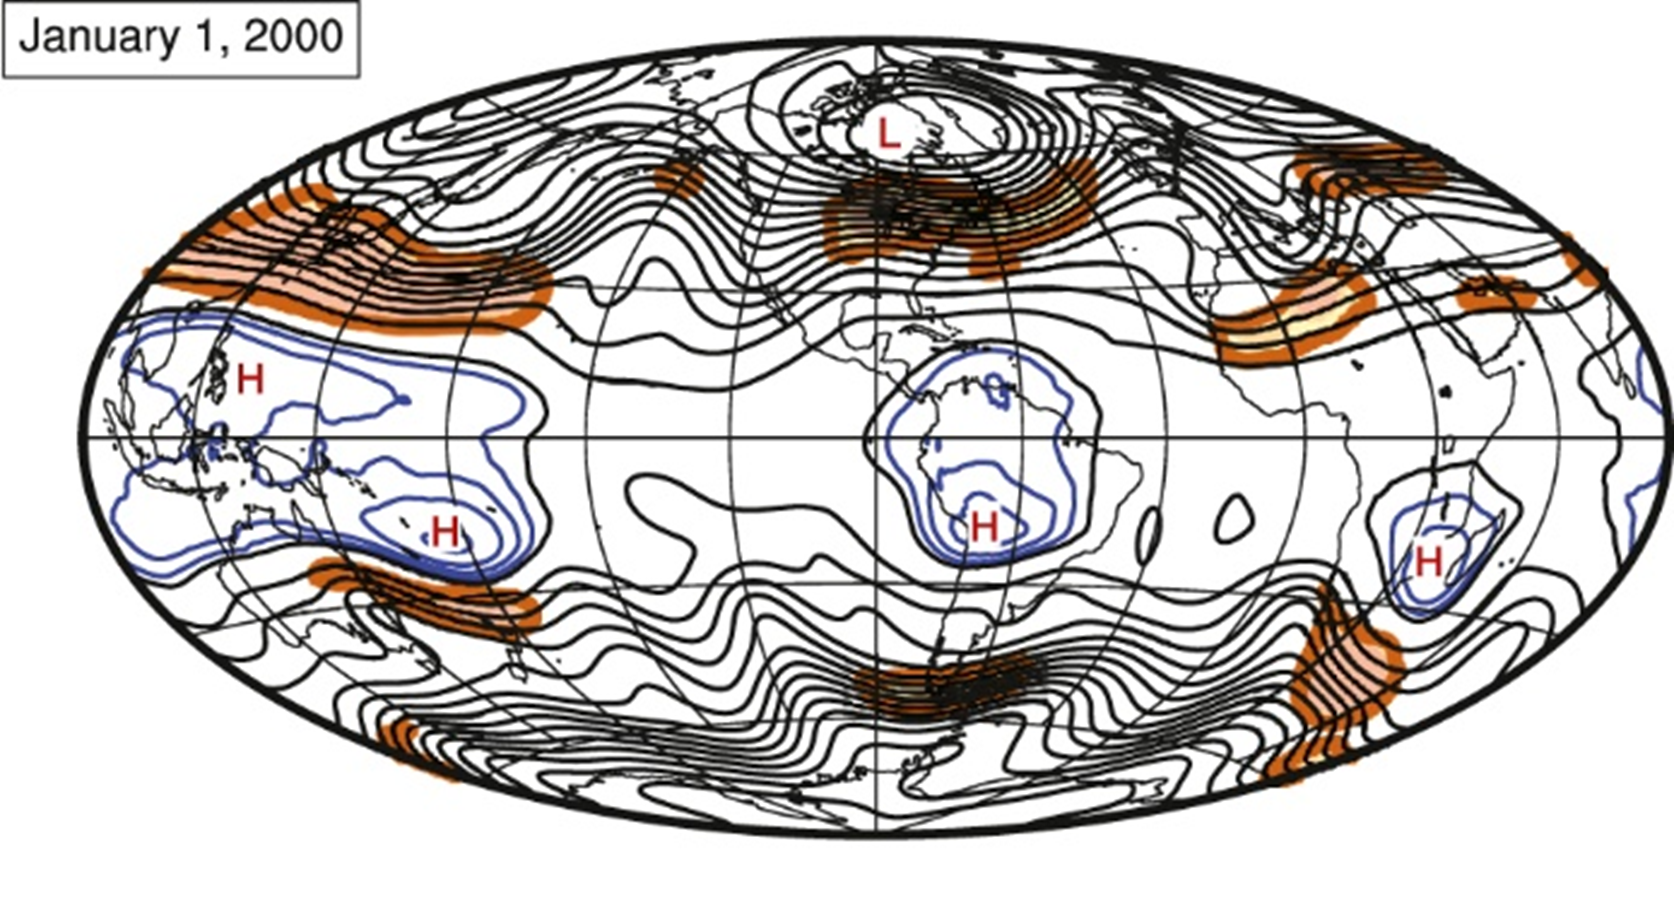
\includegraphics[width=0.5\linewidth]{uploads/geopot height.png}
    \caption{Z200 in contrasting season}
    \label{fig:geopot height}
\end{figure}
In the figure \ref{fig:geopot height}, we see the geopotential height at $200$ hPa ($\sim 8$ km), upper troposphere, that is a proxy for pressure. This picture shows where are the winds: geostrophic approximation is good for large scales (Coriolis balances pressure gradient), and where are the strongest winds: at closed isobars very strong flow ($\sim 30$ m/s)= jet stream. There are two anticyclonic ridges (H) and one through over Italy (L). If we take the average these structures disappear. Since in this graph it is january, we have summer in the SH $\rightarrow$ high pressure in the upper troposphere. 
In figure \ref{fig:summer} we can notice the a southern Asian monsoon (high pressure on tibet), jet stream gets weaker and the transient activity too. 
\begin{figure}[htp]
    \centering
    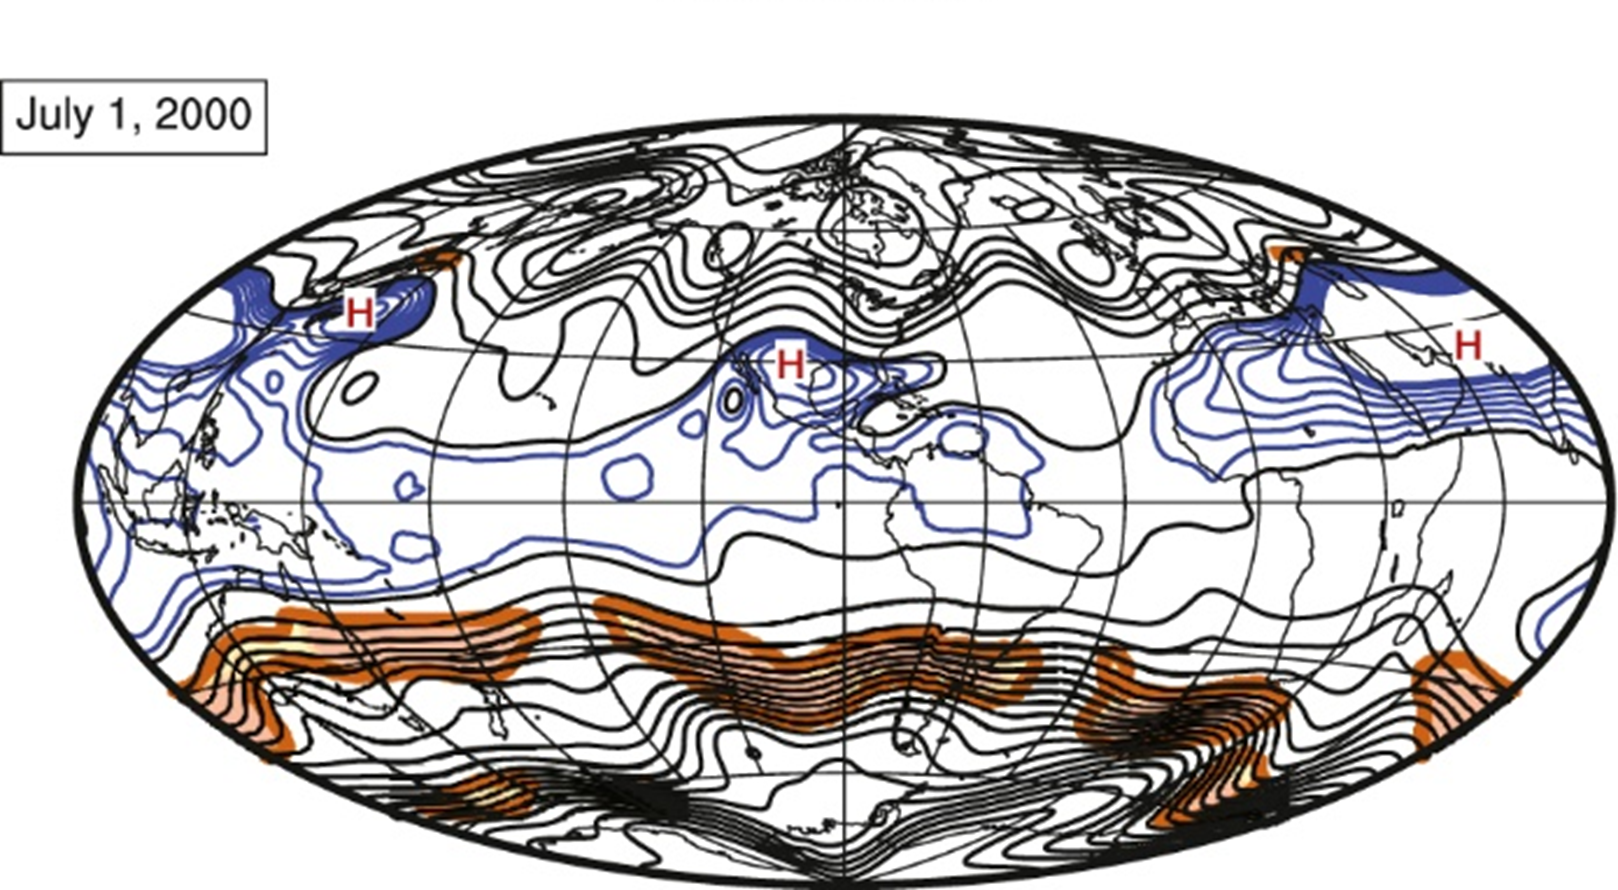
\includegraphics[width=0.5\linewidth]{uploads/summer.png}
    \caption{Z200 in contrasting season}
    \label{fig:summer}
\end{figure}

In \ref{fig:time mean} the transient disappear, we see larger symmetry in the SH and ridging and throughing over America. These meandres are due to the presence of land masses that provide differences between SH and NH in tropics. Tropics have different weather with respect to the rest of the world: here there's a superposition of Rossby and Kelvin waves due to heating associated with land. 
\begin{figure}[h]
    \centering
    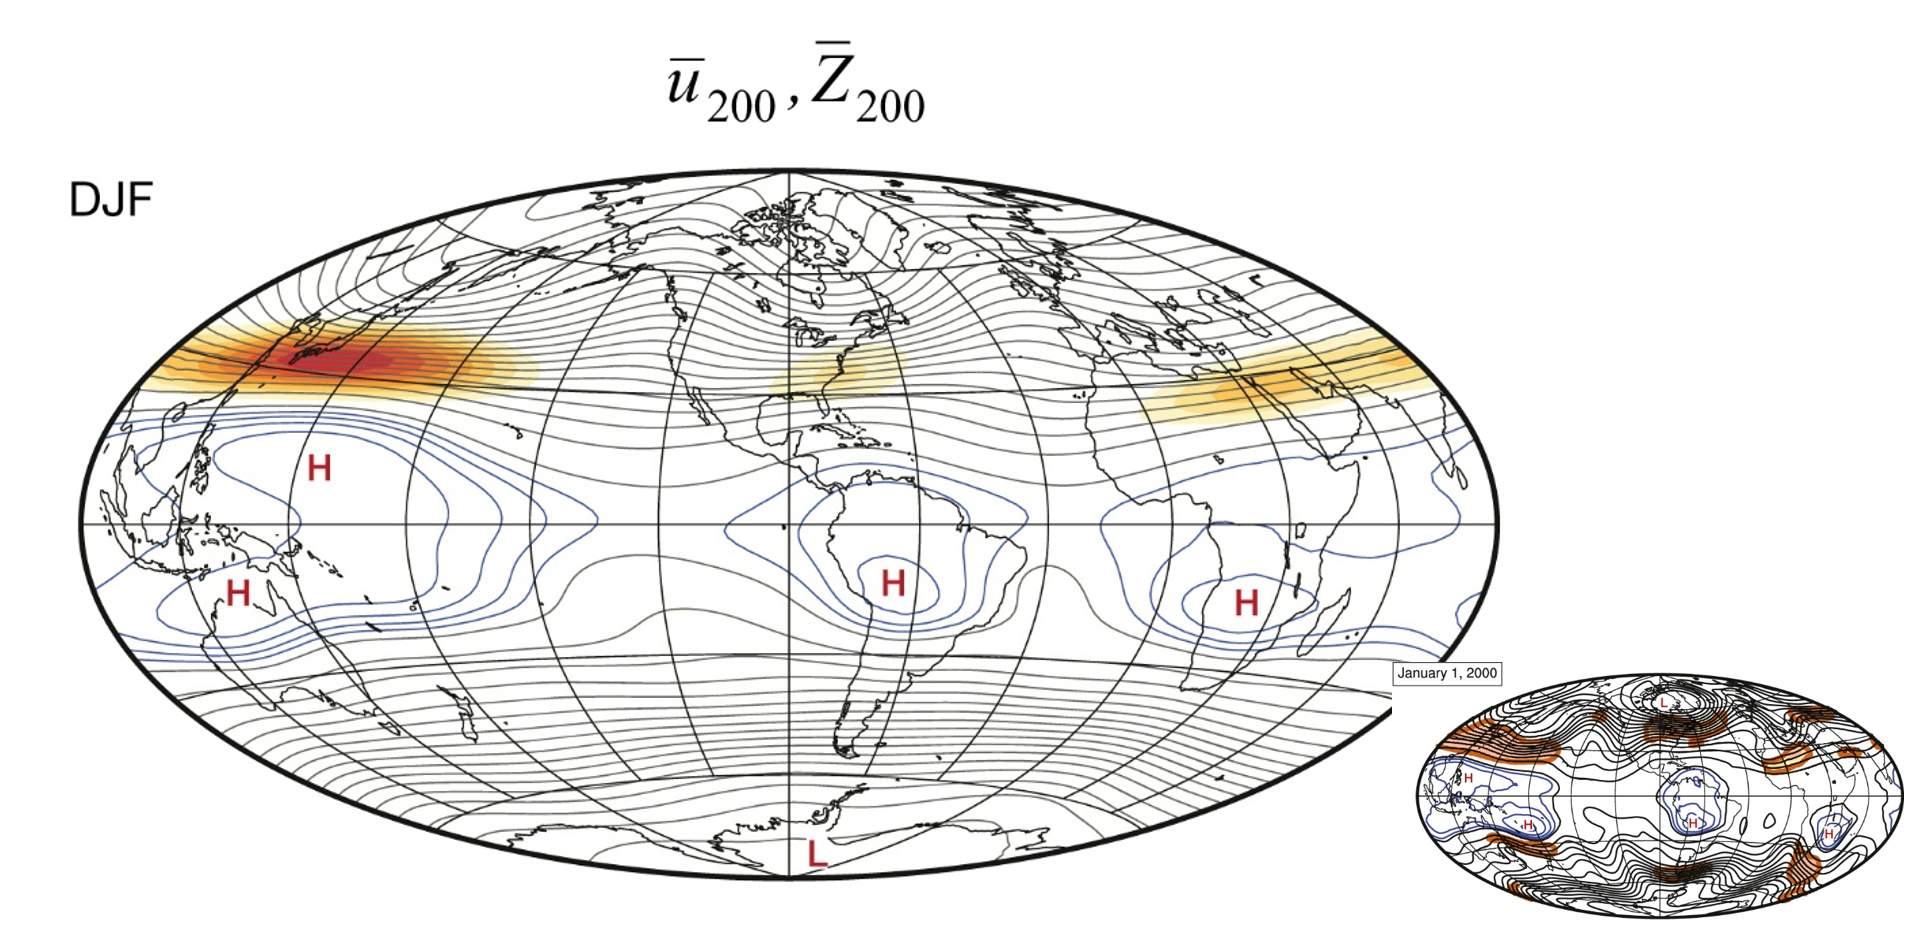
\includegraphics[width=0.65\linewidth]{uploads/time mean.png}
    \caption{Time mean. Transient disappears; larger symmetry in SH; ridging and throughing over America}
    \label{fig:time mean}
\end{figure}
In \ref{fig:skewT} the difference between location at the same $\lambda$ (points over land are colder than ocean ones:)$\rightarrow$ different heat capacity. 
\begin{figure}[h]
    \centering
    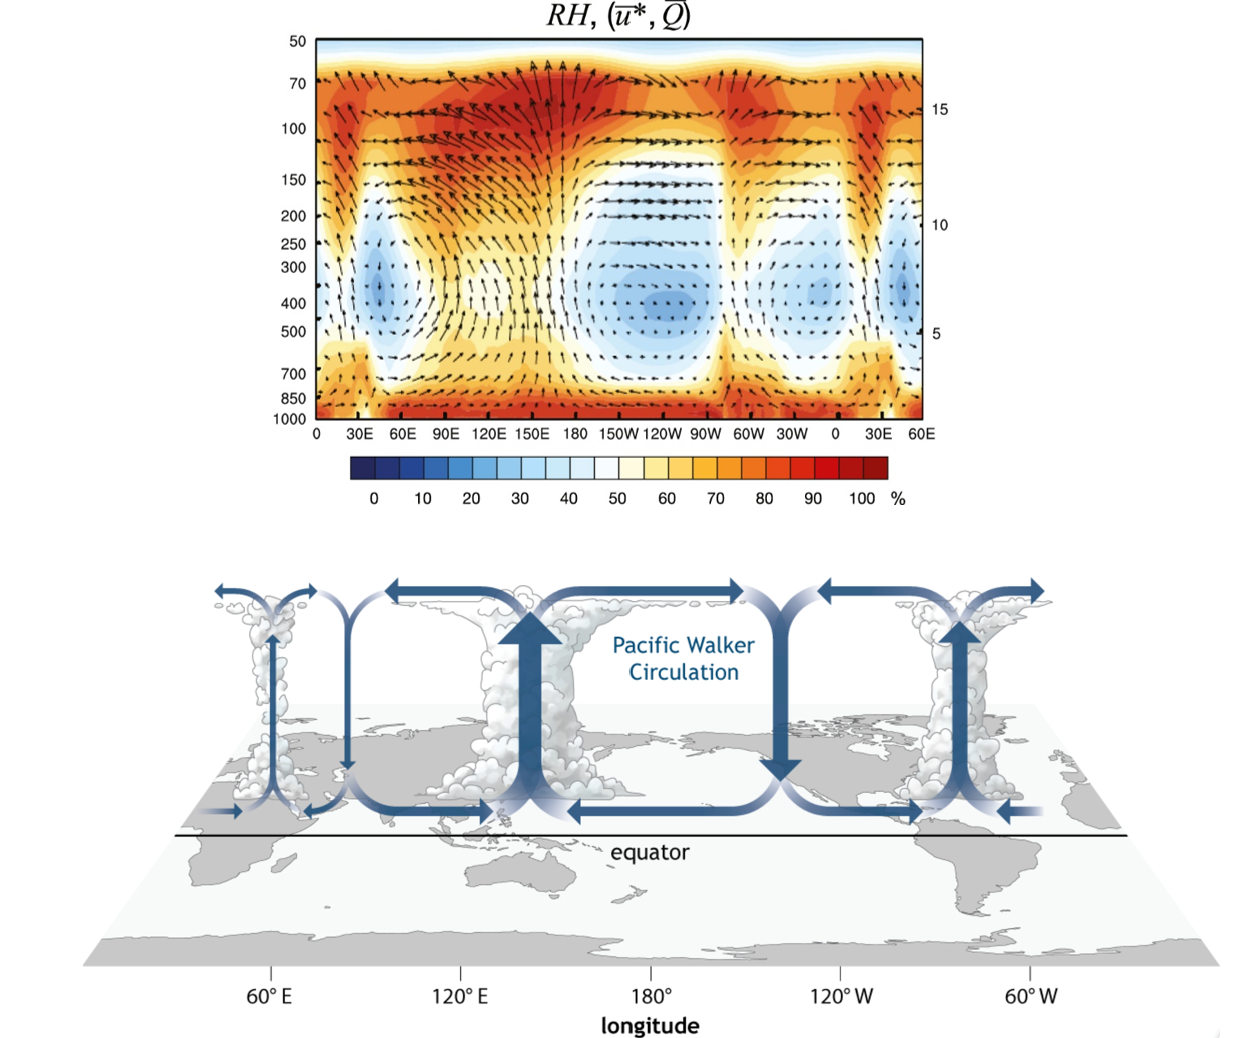
\includegraphics[width=0.5\linewidth]{uploads/sket T surface.png}
    \caption{Skin Temperature surface}
    \label{fig:skewT}
\end{figure}
\begin{wrapfigure}{r}{0.5\textwidth} %this figure will be at the right
    \centering
    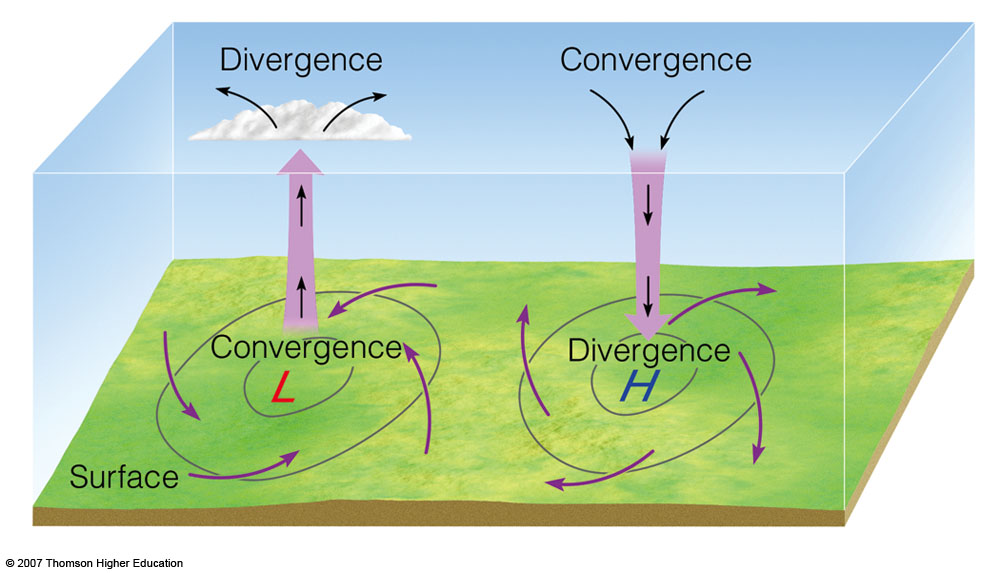
\includegraphics[width=0.59\linewidth]{uploads/H and L.png}
    \label{fig:HL}
\end{wrapfigure}
Fig. \ref{fig:SLP} shows on average annually and seasonally the distribution of sea level pressure and near surface winds. The friction of the surface adds to the pressure force and Coriolis force (H vs L pressure zone). Because of geostrophic balance the friction of the surface acts on the pressure force, curving a bit the isobars; that's why you have a convergence on the Low pressure zones and a divergence on the Highs, as in fig.\ref{fig:HL}.





\begin{figure}[h]
    \centering
    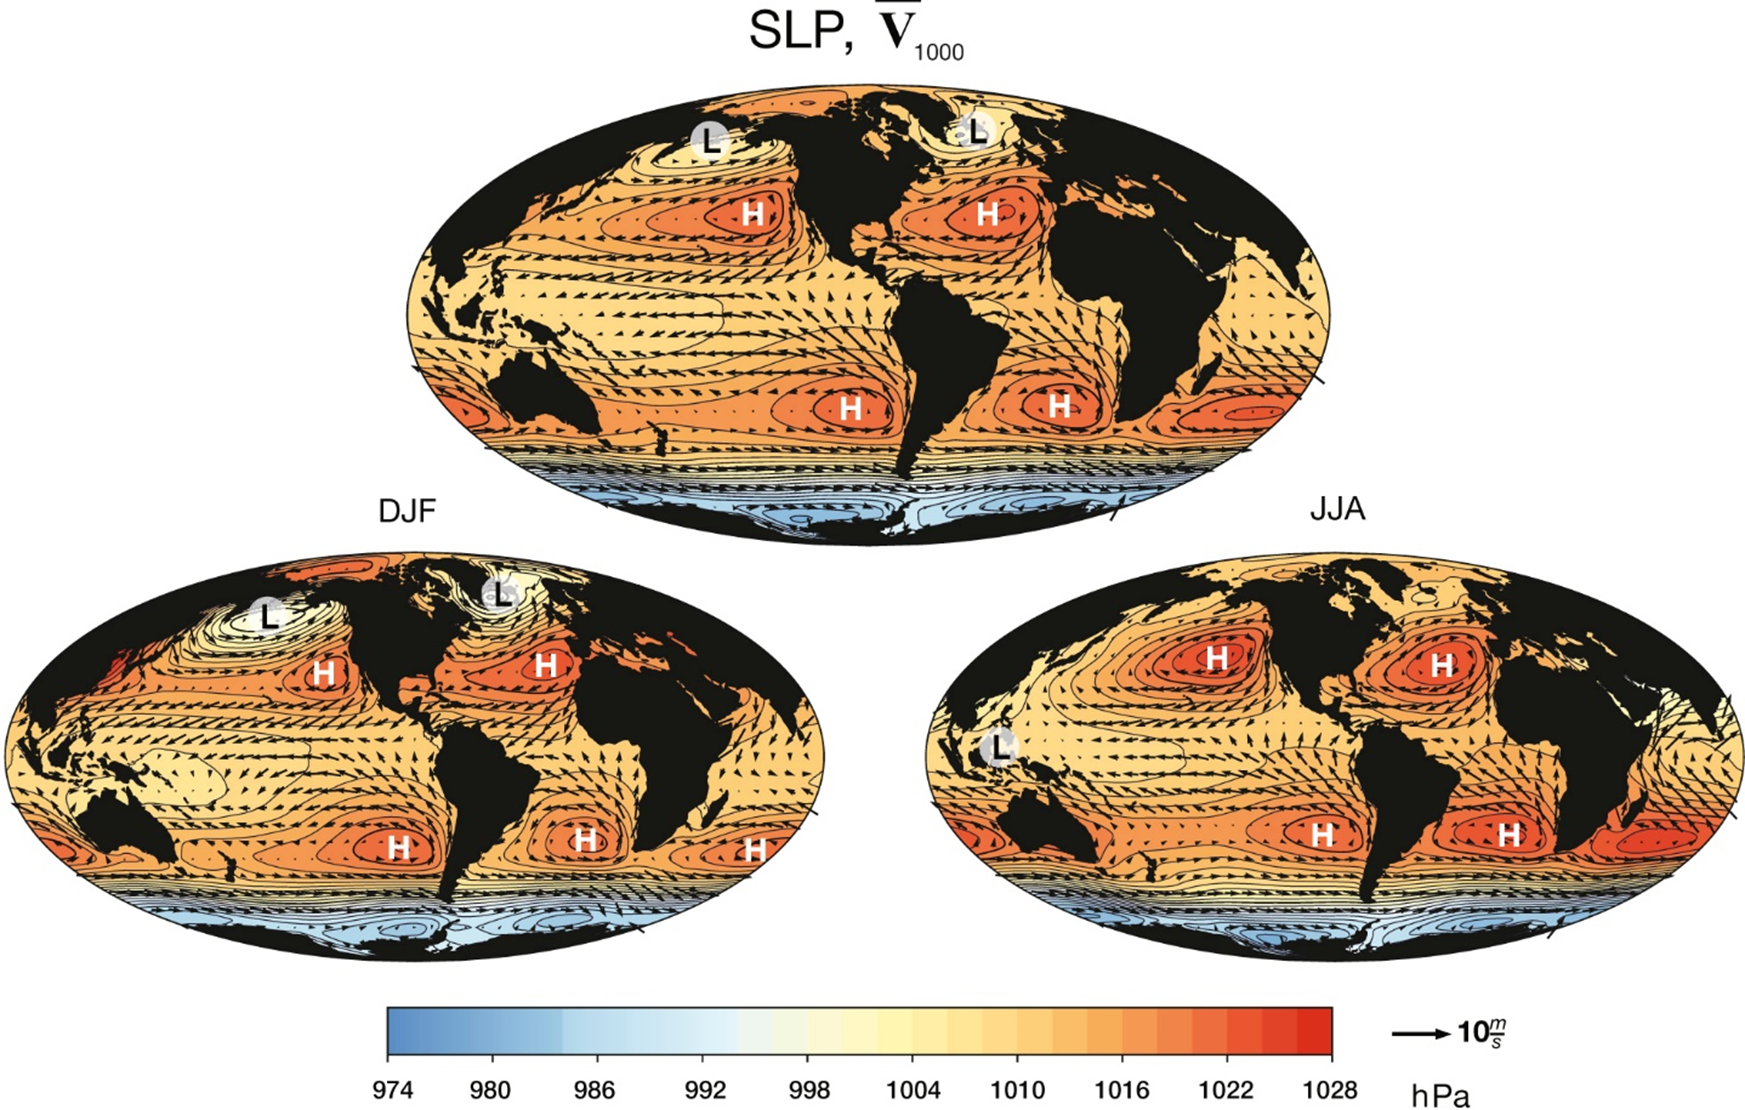
\includegraphics[width=0.5\linewidth]{uploads/SLP.png}
    \caption{Distribution of sea level pressure.}
    \label{fig:SLP}
\end{figure}








Annual mean: average over the all months: the upper figure of \ref{fig:SLP}: westerly (they come from the west, they go eastward) winds North Atlantic Pacifical High (same heaven subtropical high). In the Northen Hemisphere you have two semipermanent low pressure  areas semipermanent Atlantic low, (semipermanent Icelandic Low). Subtropics semipermanent high pressure and semipermanent low pressure at high latitude forces the winds to be westerly. In the tropics winds are easterly: trade winds, in the Equator they tend to converge driven by high pressure systems. Where does the easterly turns into westerly? 30° is this boundary,  constant as a consequence of the atmospheric angular momentum. 
\begin{figure}[htpb]
    \centering
    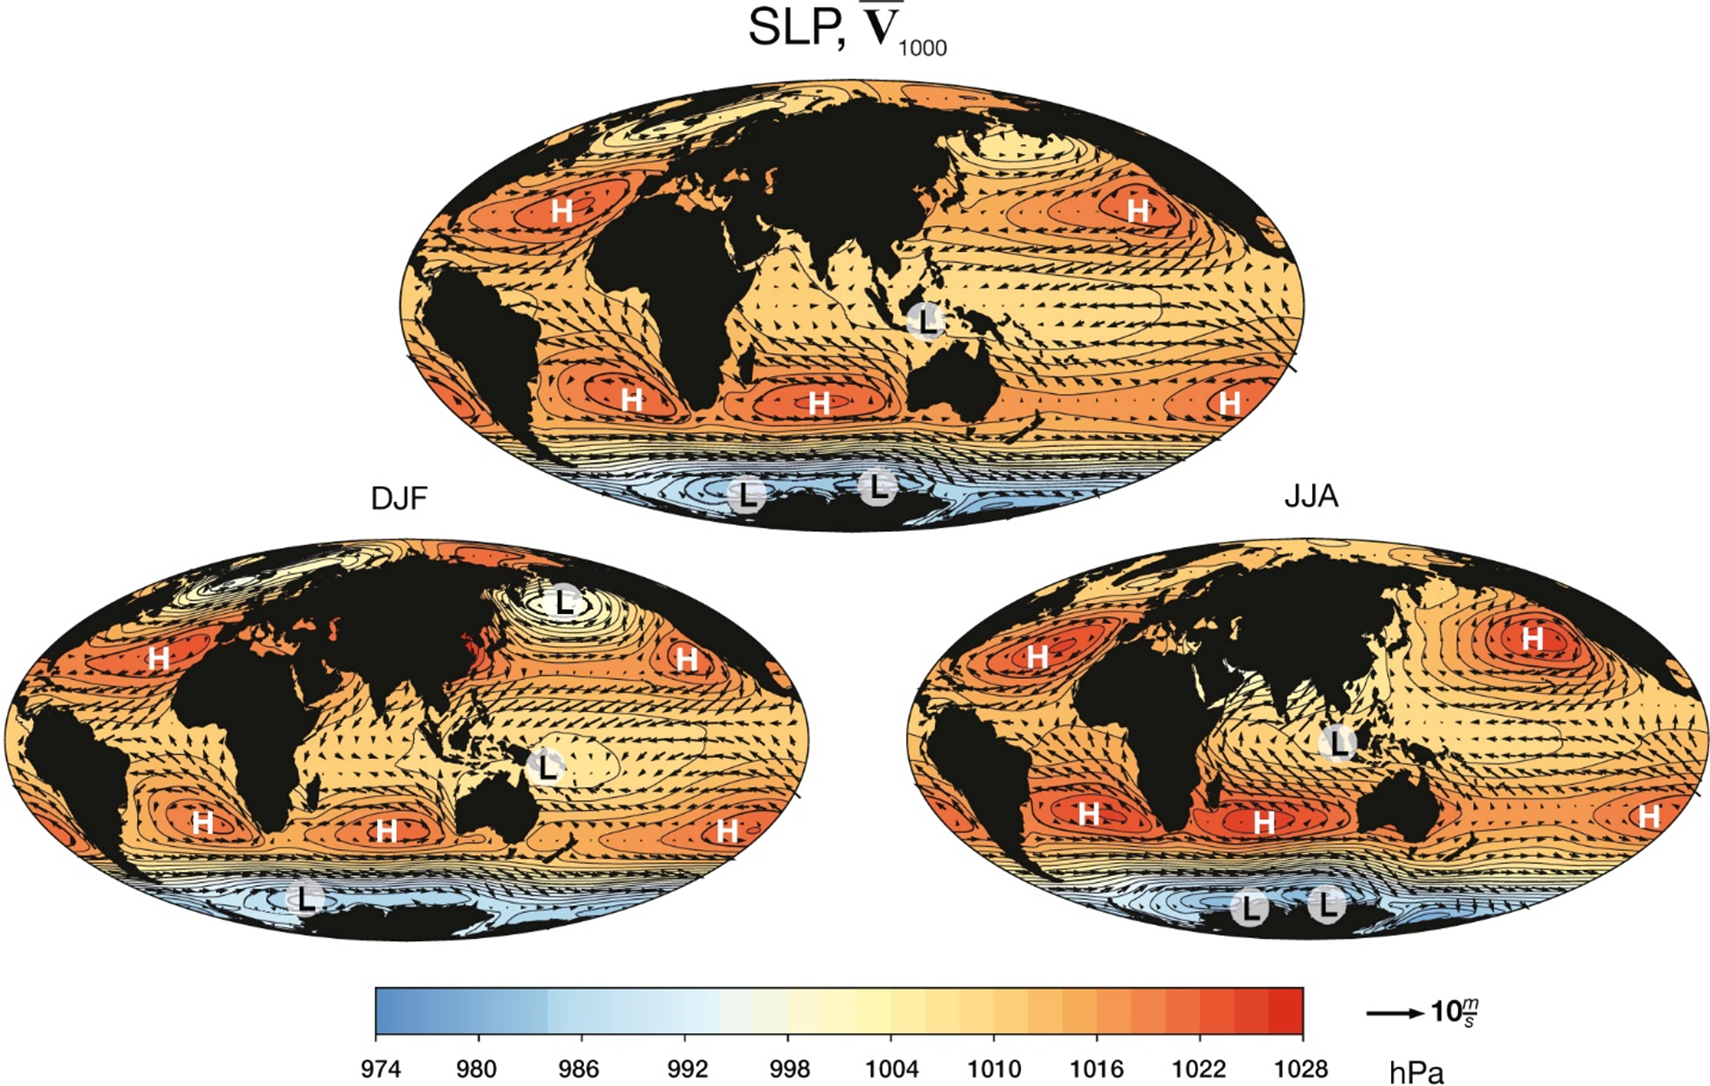
\includegraphics[width=0.5\linewidth]{uploads/SLP centered in Asia.png}
    \caption{SLP centered in Asia}
    \label{fig:SLP Asia}
\end{figure}
Fig.\ref{fig:SLP Asia} is centered in the continental mass of Asia. During winter, winds blow from the continental mass towards the Indian Ocean, in summer they move in the opposite way: Somali jet towards Somalia. This large deviation is due principally to the Asian continental mass. NB: Seasonally, wind reversal means monsoon. The continent plays a very important role in shaping winds. 
\begin{figure}[htpb]
    \centering
    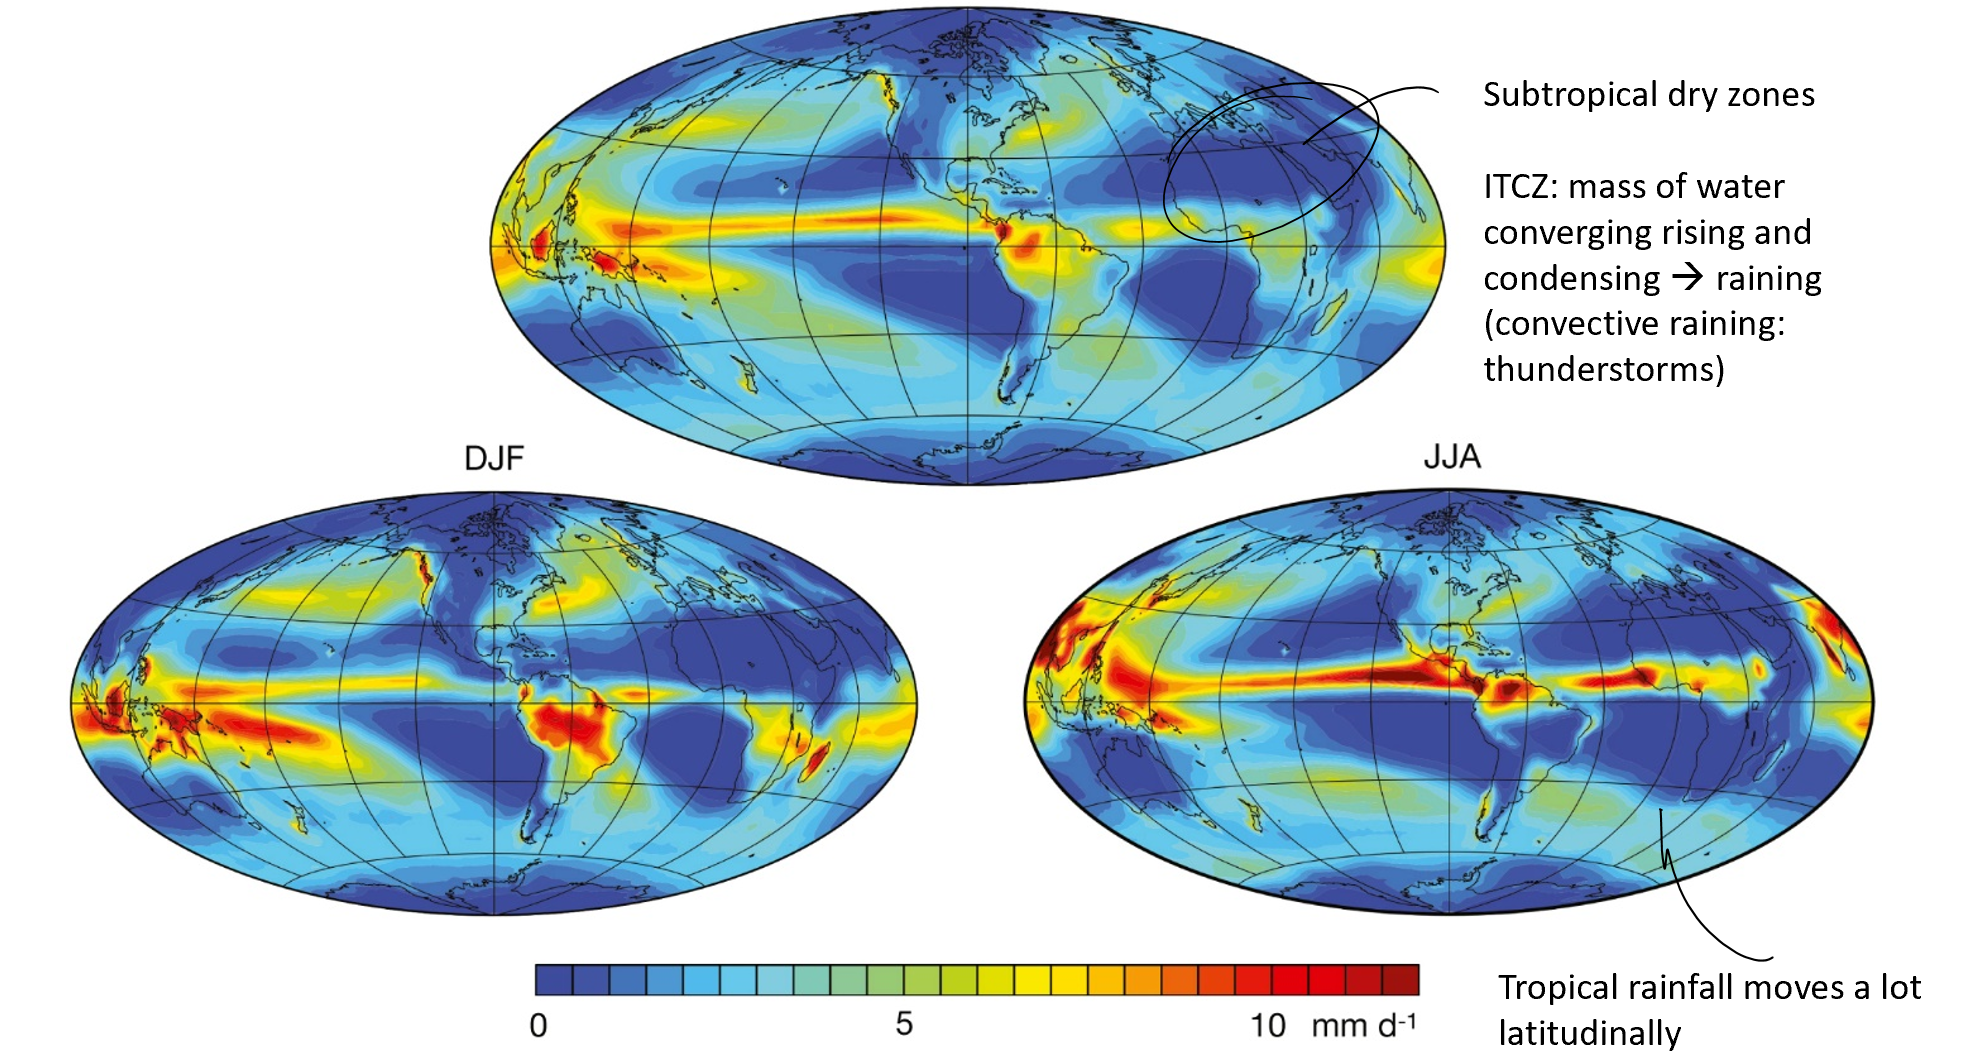
\includegraphics[width=0.5\linewidth]{uploads/Precipitation.png}
    \caption{Annual mean of precipitation. How much precipitation falls on average on a year (or season) for every grid point.}
    \label{fig:precipit}
\end{figure}
Areas under the high pressures are called subtropical dry zones, where there's very little precipitations, over the ocean there is area with high precipitation, winds converge in the ITCZ (around 7°N) stable seasonally.
DJF large amount of rainfall in the South of the Equator, while in the opposite season this area gets completely dry, the rainfall largely shifts northward. 
\begin{figure}[htpb]
    \centering
    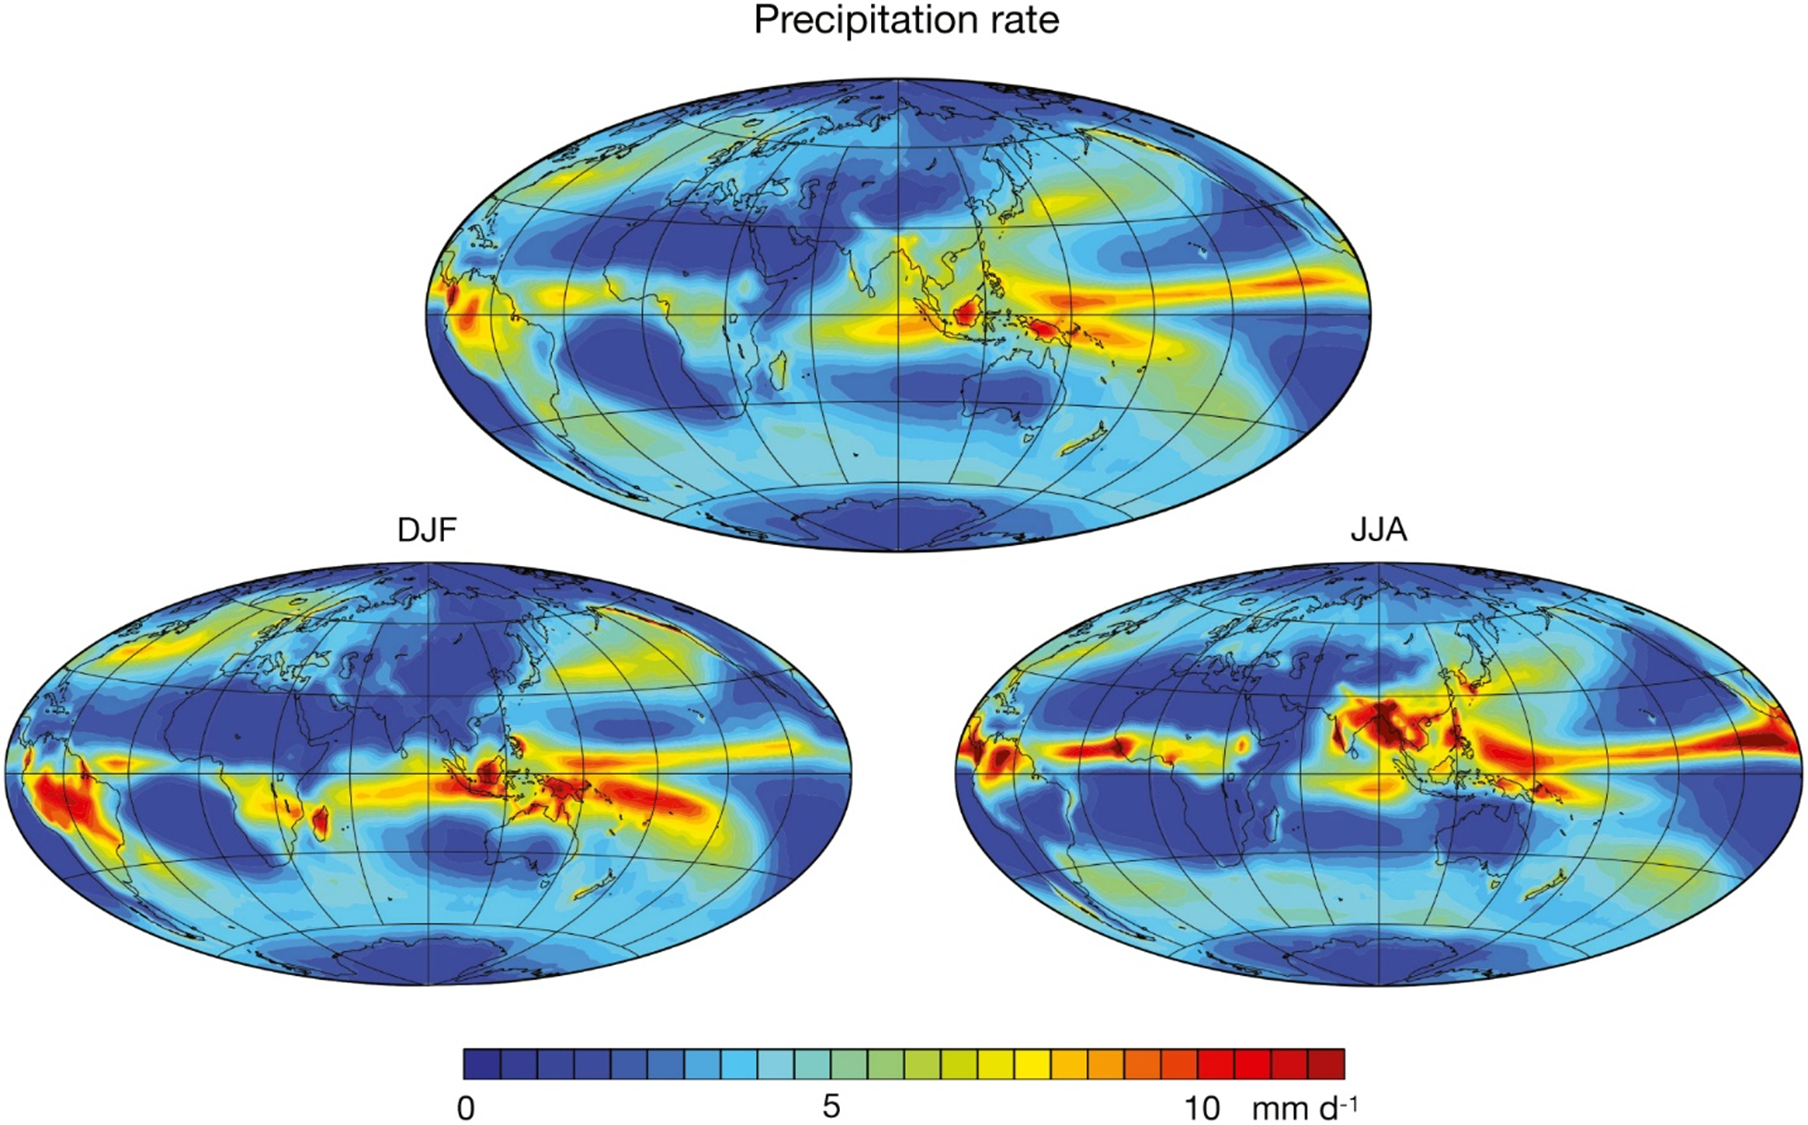
\includegraphics[width=0.5\linewidth]{uploads/precip Asia.png}
    \caption{Annual mean of precipitation centered in Asia}
    \label{fig:precipit Asia}
\end{figure}
The seasonal shift of the tropical Asian monsoon (from Pakistan up to Korea) in the tropics means that you have areas that are dry; over the ocean the ITCZ does not move, in correspondence of the large continental masses, the rain follows the seasons: high in summer, and it shifts largely in terms of degrees up to 10m of rain per year.\\


If you look at extra tropics (30°N or S), there is another belt where precipitation is high (not high as tropics). Fig.\ref{fig:precipit} shows better the continuous belt in extra tropics; this rain is associated with the fact that lots of cyclones form close to USA, meaning there are rainfalls completely different than Indian monsoon, these are \textbf{extra tropical cyclones}. These cyclones tend to form over preferential places and move over preferential zones, they are modulated seasonally: for example in winter these cyclones are more intense. The track where preferentially extra tropical cyclones tend to move (the reason why in England it rains a lot) is called the \textit{ extra tropical storm track}. Any circulation that is closed is a cyclone, they divided in two kinds: 
\begin{itemize}
    \item \textit{extra tropical cyclones} associated with baroclinic instability, they are responsible for most of the rain and tend to move over extratropical storm tracks.
    \item \textit{tropical cyclones} (also called hurricanes in North America and typhoons in Asia) associated with very warm SST and heat transfer to the atmosphere.
\end{itemize}

Due to extra tropical cyclone movement, you have a strong maximum associated with ITCZ in the equator and another maximum associated with extra tropical tracks as in Fig.\ref{fig:precipit}. 
Winds are fundamental in understanding the movement of water masses, oceans are the source of energy that keep hurricanes. 

ITCZ intertropical convergence zone. Most people indicate it to be over the oceans and monsoon just over land because they are different: ITCZ stays constant, and monsoon changes over continuous lands shifting a lot between seasons.
\begin{figure}[htpb]
    \centering
    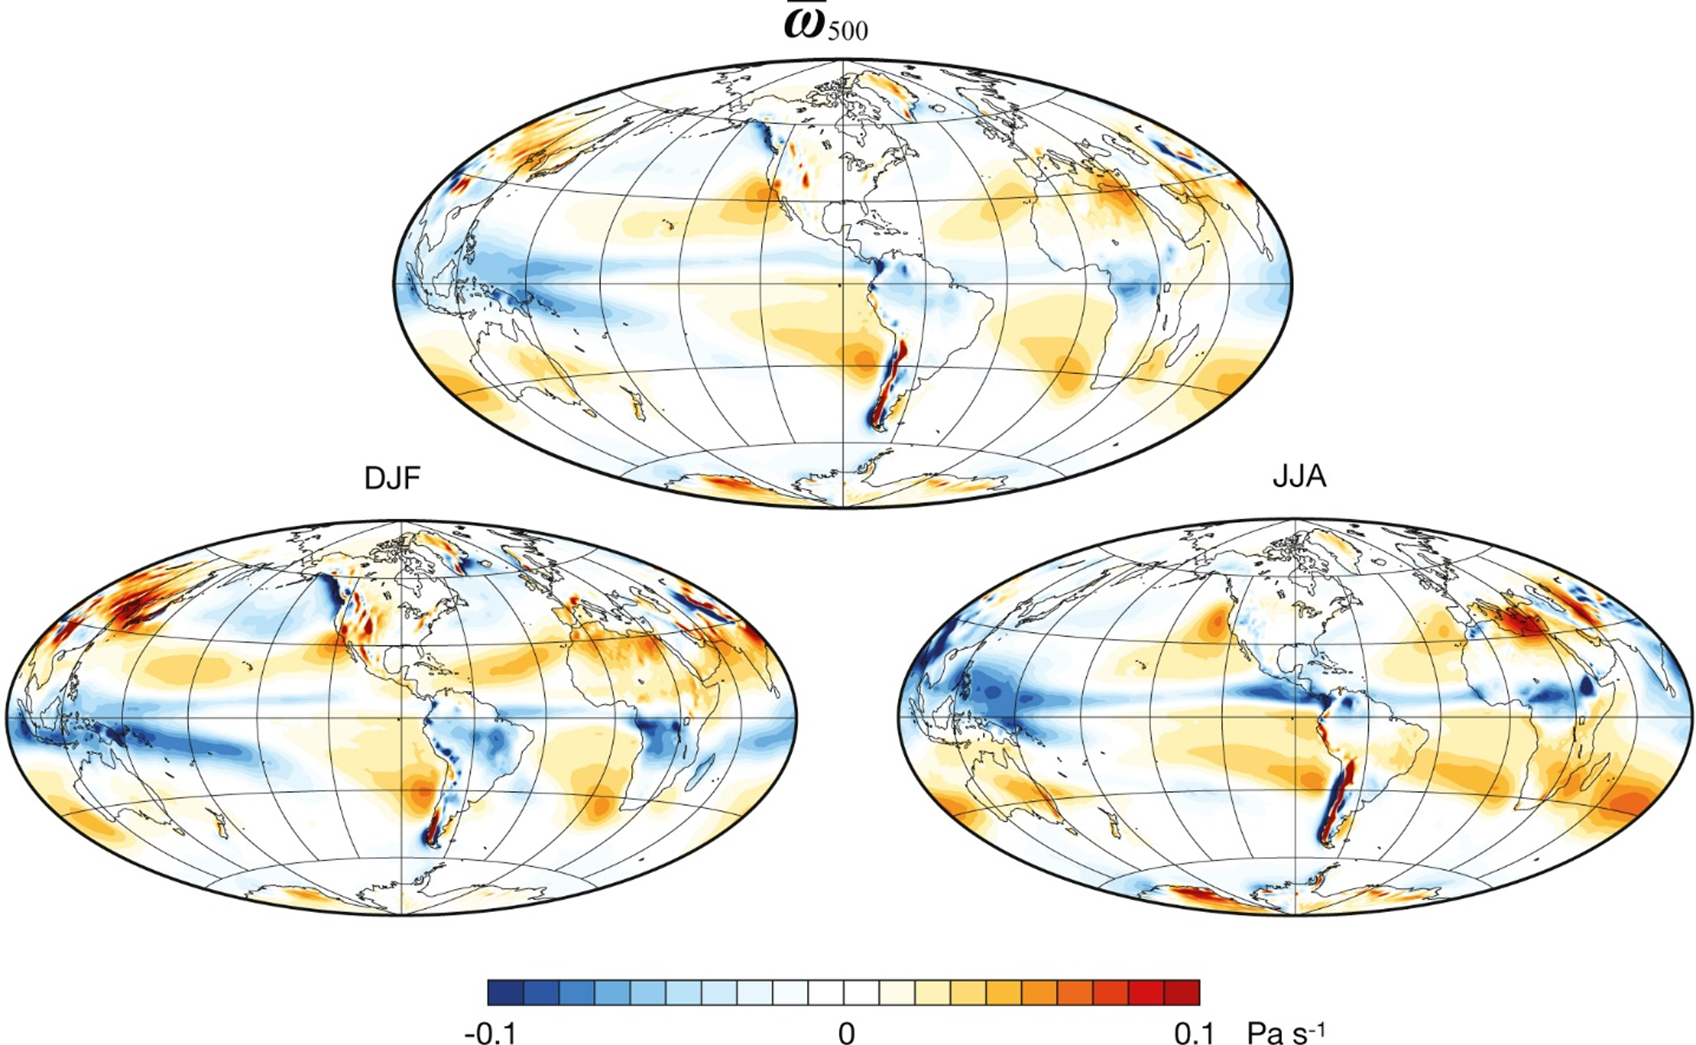
\includegraphics[width=0.5\linewidth]{uploads/Vertical p.png}
    \caption{Vertical pressure level at 500 hPa: $\omega$ is the vertical velocity in $p$-coordinates.}
    \label{fig:omega500}
\end{figure}
In fig. \ref{fig:omega500} we are in the middle of the troposphere. We see an up-welling and down-welling motion. Negative $p$ coordinate velocity ($\omega$) means an upwelling motion (upward motion) because height grows while the pressure decrease; positive omega down-welling motion makes sense as you're carring moisture away. We can say the mean vertical velocity in pressure coordinates $\omega$ is a proxy for precipitations as it correlates quite well with fig.\ref{fig:precipit} in the tropics (areas of large precipitation related to negative $\omega$) but not in the mid latitudes. This is because tropical rainfall are associated with a mean circulation that is persistent (all days uprising motion); in storm tracks we have cyclones continually reforming and replaced by anticyclones (downward motion), meaning that on average they cancel out (they are transient): the rainfall in the extra tropics is associated with a transient phenomena: averaging it goes to zero. Fundamental difference: in tropics precipitation is associated with mean circulation, in extra tropic precipitation is associated with transient: you don’t see them in mean, you have to take quadratic terms like stand deviation in order to see them. \\
[0.25 cm]


Until now we considered time means fixing some height (surface, $500$ hPa, \dots) without really focusing on how things vary with height. To analyse this we should look at 3D, a bit complicated, an easy way to look how things depend on height is to look zonally. Remember that zonal mean implies averaging along circles having the same latitude, by doing that you compress the longitudinal dimension and in a 3D field you get to work only with latitude and height. As we said the main properties of the atmospheric circulation at first order depend on latitude, they also depend on longitude but higher order. 

Fig.\ref{fig:zonal mean} shows the zonal mean of the time mean zonal wind (component along the parallels). Winds increase with height in the extra tropics and has a maximum value around the same 10 km: the two cores in the S and N hemisphere jet streams. 
In the stratosphere it is different: you don't have two westerly jets ($u$ positive means it grows from West towards East), there is a stronge easterly jet in the polar \textit{polar night jet} observed. Close to the surface the transition from westerly to easterly is preatty stable across the season and it is 30°. The jet in the winter is stronger in the NH, due to the thermal wind balance that relates the gradient of $T$ at surface with the shear of the wind (large in winter than in summer).

\begin{figure}[htpb]
    \centering
    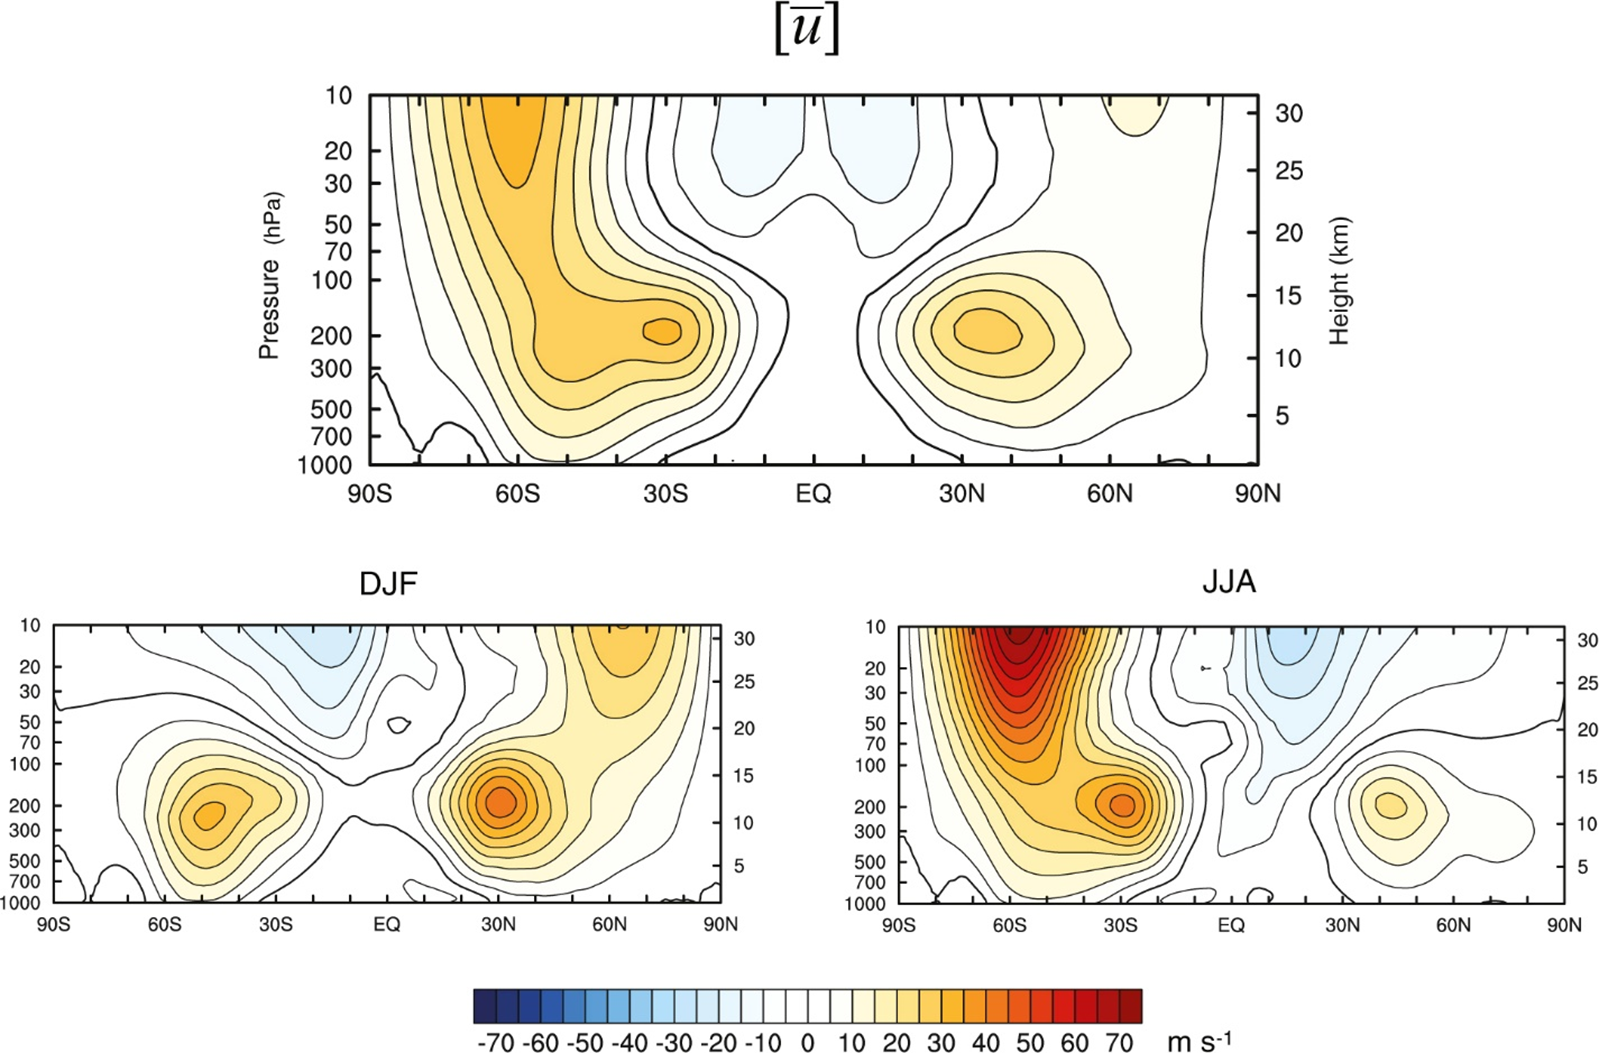
\includegraphics[width=0.5\linewidth]{uploads/Zonal mean.png}
    \caption{Zonal mean of the time mean zonal wind.}
    \label{fig:zonal mean}
\end{figure}



\begin{figure}[htpb]
    \centering
    \includegraphics[width=0.45\linewidth]{uploads/thermal structure.png}
    \caption{Thermal structure of the atmosphere}
    \label{fig:thermal structure}
\end{figure}
Fig.\ref{fig:thermal structure} shows the thermal structure of the atmosphere. You have average everywhere worldwide. In troposphere $T$ decreases: this rate is the vertical lapse rate $\Gamma=-dT/dz$, about $6.5$ K km$^{-1}$: similar to what the moist (or saturated) lapse rate predicts (dry lapse rate is steeper $\sim 10$ K km$^{-1}$), because of water vapor (condenses when it rains) the real lapse rate is less. This means that on average the lapse rate in the global troposphere is controlled by the saturated lapse rate, in the tropics especially: lots of rainfall. \\
[0.2 cm]

From fig.\ref{fig:vert structure of T}, we see that temperature overall decreases when you go from the surface up to the tropopause and it decreases when you move from the tropical regions poleward. In the tropics temperature doesn't vary much, while in the extra tropics you have a large gradient $\leftrightarrow$ tropospheric jet streams are placed here: here there's the largest meridional temperature gradient and because of the thermal wind balance this is consistent with a vertical wind shear (wind grows very rapidly in the jet core where there's large thermal gradient).
\begin{figure}[htpb]
    \centering
    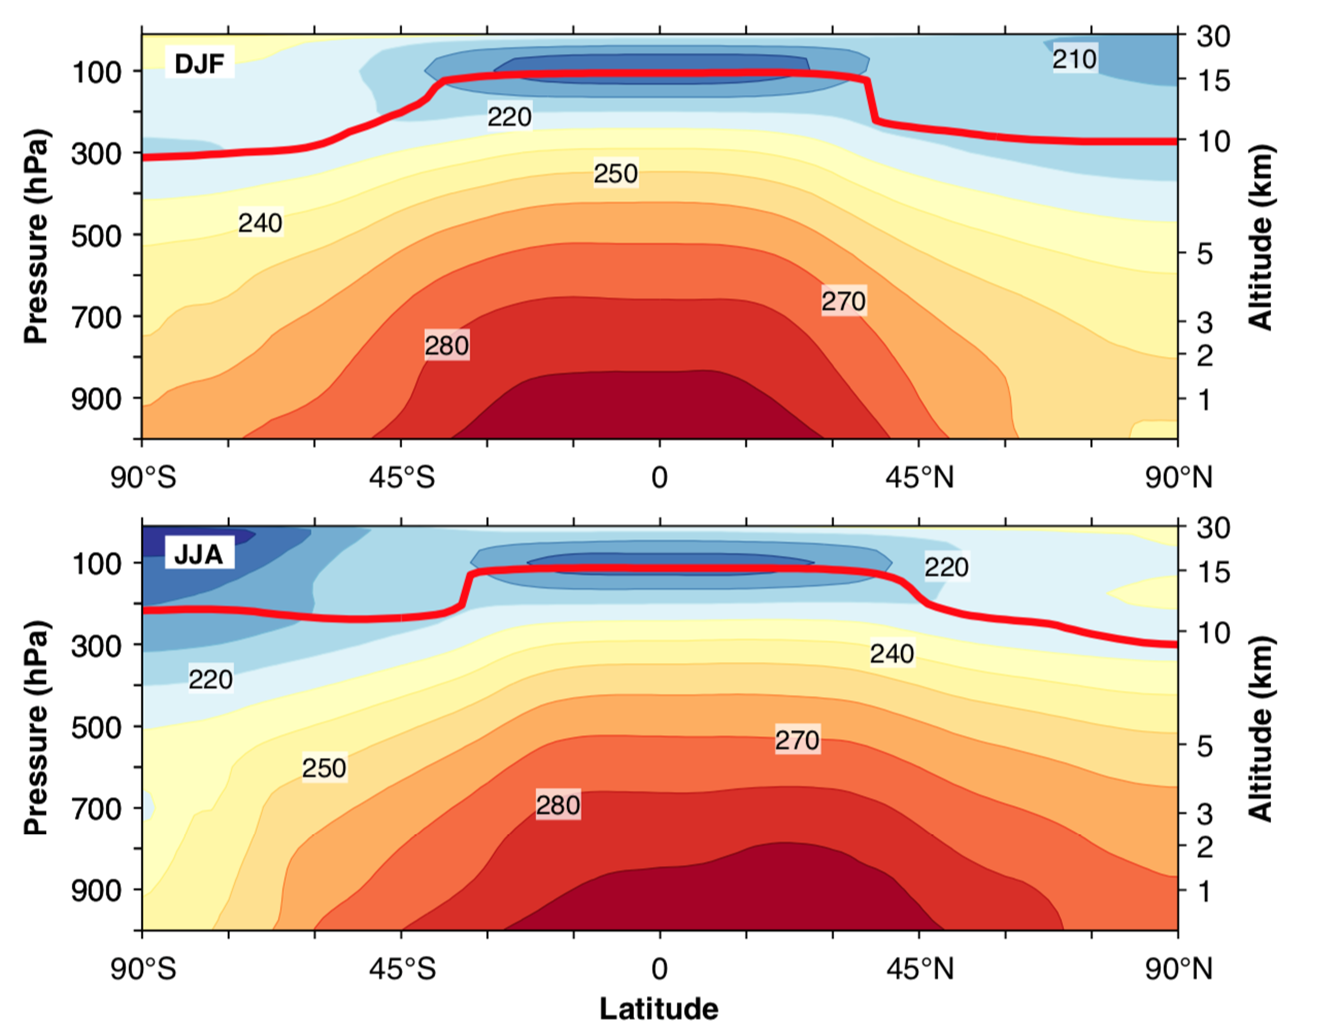
\includegraphics[width=0.5\linewidth]{uploads/Thermal structure.png}
    \caption{Vertical structure of temperatures in the zonal mean.}
    \label{fig:vert structure of T}
\end{figure}


Now let us look at where water vapor is in the atmosphere. The concentration of water vapor is very high near the surface and near the Tropics, it drops moving upward. The zonal mean of specific humidity closely mirrors the distribution of temperature. Where is warmer you have the highest concentration of water vapor. 
\begin{figure}[htpb]
    \centering
    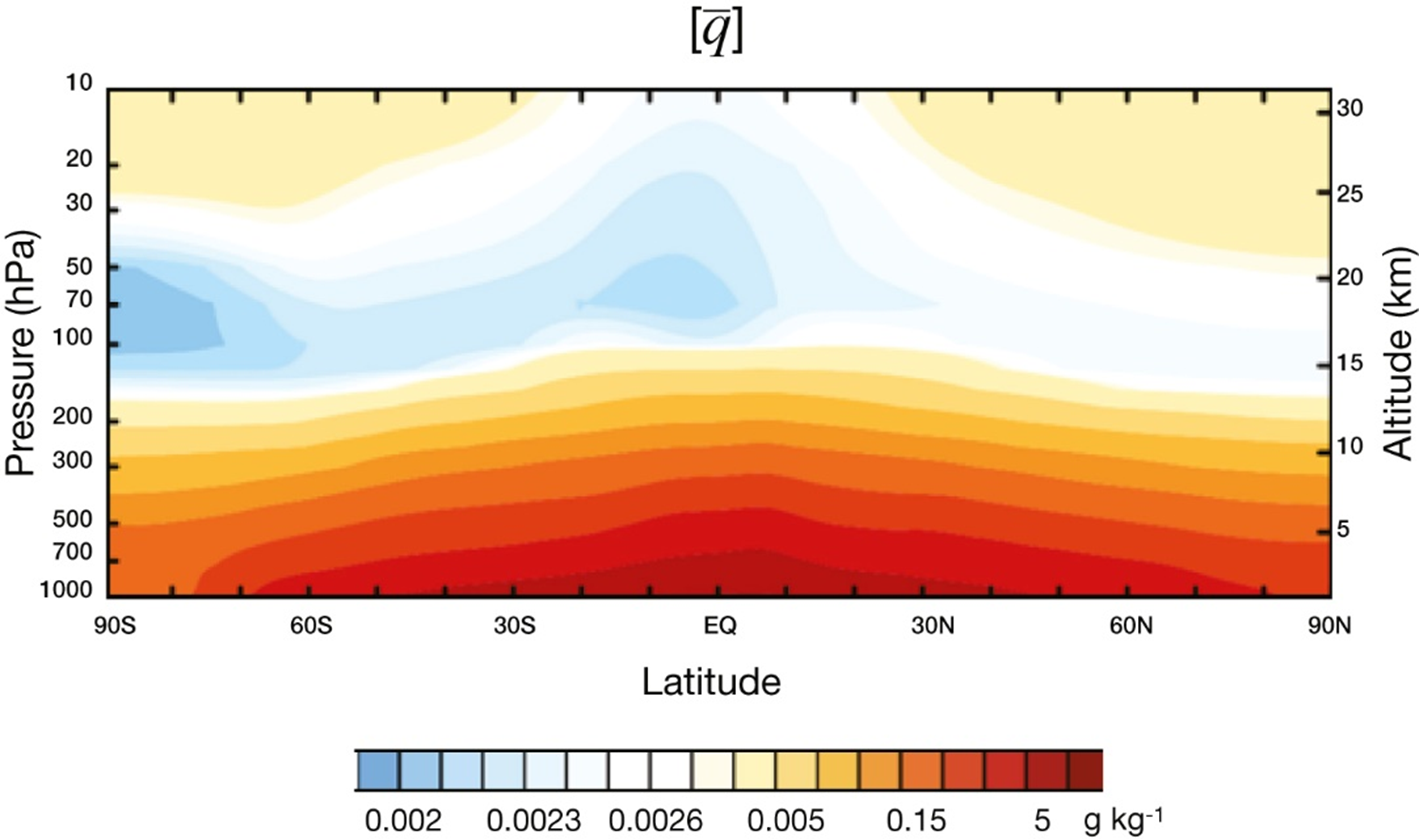
\includegraphics[width=0.5\linewidth]{uploads/specific humidity.png}
    \caption{Zonal mean of specific humidity: where water vapor is in the atmosphere.}
    \label{fig:specific humidity}
\end{figure}
The relationship between temperature and humidity is expressed by the Clausius-Clapeyron relation, which expresses for each degree of warming how much water vapor we will have. Related to an increase in precipitation extremes. The concentration of water vapor drops as you move upward and upward. Clausius-Clapeyron relation relates the concentration of water vapor to temperature:
\begin{equation}\label{eq:CC eq}
    \frac{dq_s}{q_s}\simeq \color{RawSienna}\left(\frac{L}{R_vT^2}\right)\color{black}dT
\end{equation}
where on the left there's the relative change of specific humidity, the \textcolor{RawSienna}{fraction} on the right is the relative latent heat proportional to a variation in temperature and to $R_v$ gas constant for water vapor, with $L\simeq 2.5 \quad 10^6$ J/K, $R_v\simeq 461$ J/(K kg) and $T\simeq 300$ K $\simeq 20$ °C, we obtain a proportional factor $\alpha \simeq 7\%$, meaning that for every $1$°C warming, the relative humidity increases of $7\%$.
\begin{figure}[htpb]
    \centering
    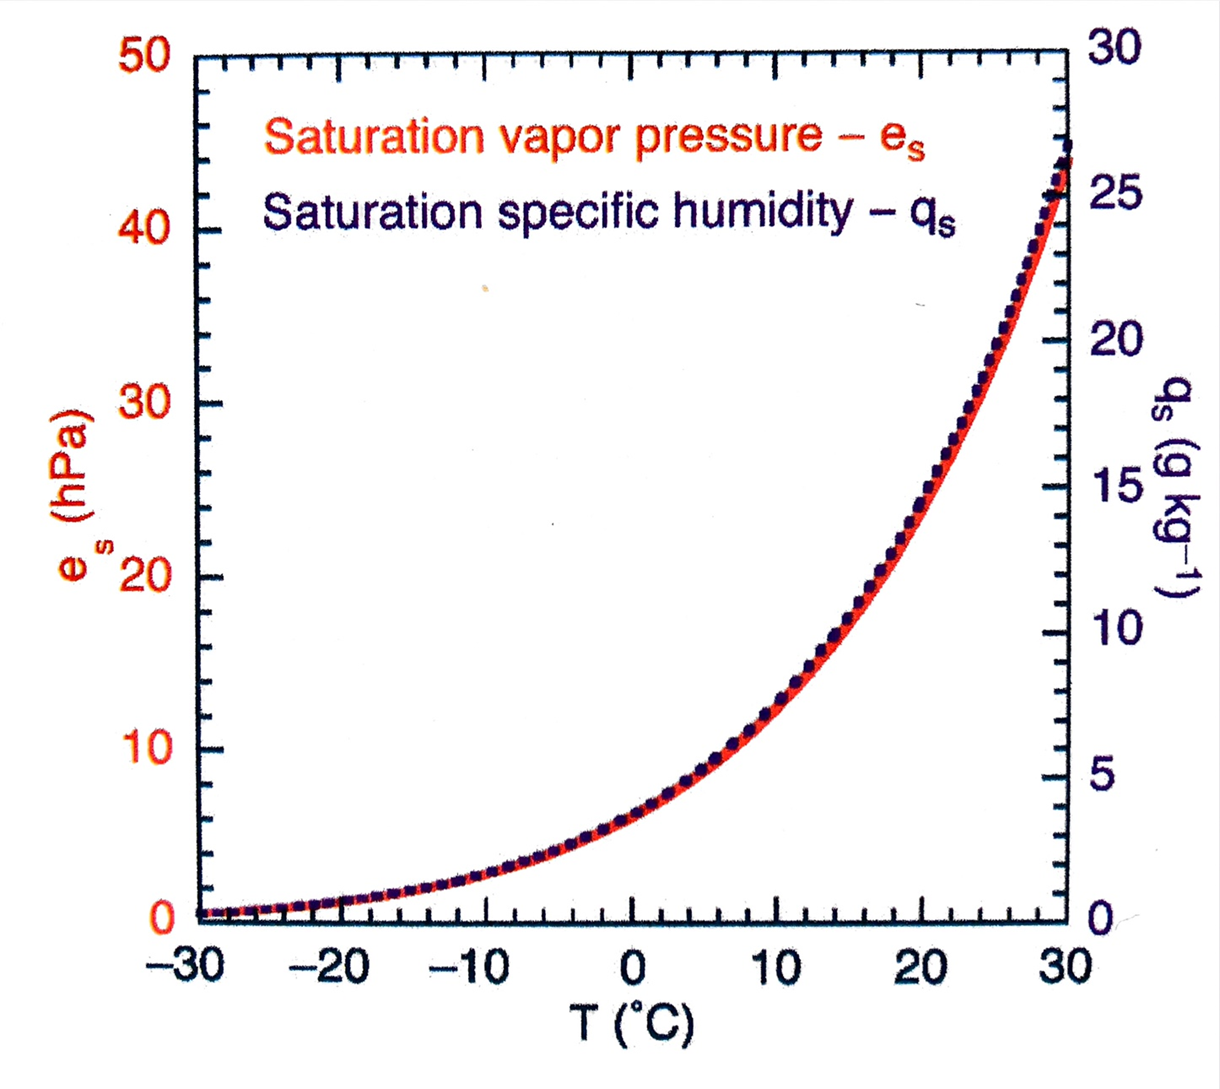
\includegraphics[width=0.5\linewidth]{uploads/exact CC.png}
    \caption{Exact solution of the Clausius-Clapeyron equation. NB in very cold conditions the atmosphere is dry.}
    \label{fig:exact CC}
\end{figure}

This plot shows zonal mean time mean meridional velocity. Around the Eq there’s an area with large ascent. Two meridional circulations associated with Hadley cells. There’s a better way to see: the meridional stream function. 
\begin{figure}[htpb]
    \centering
    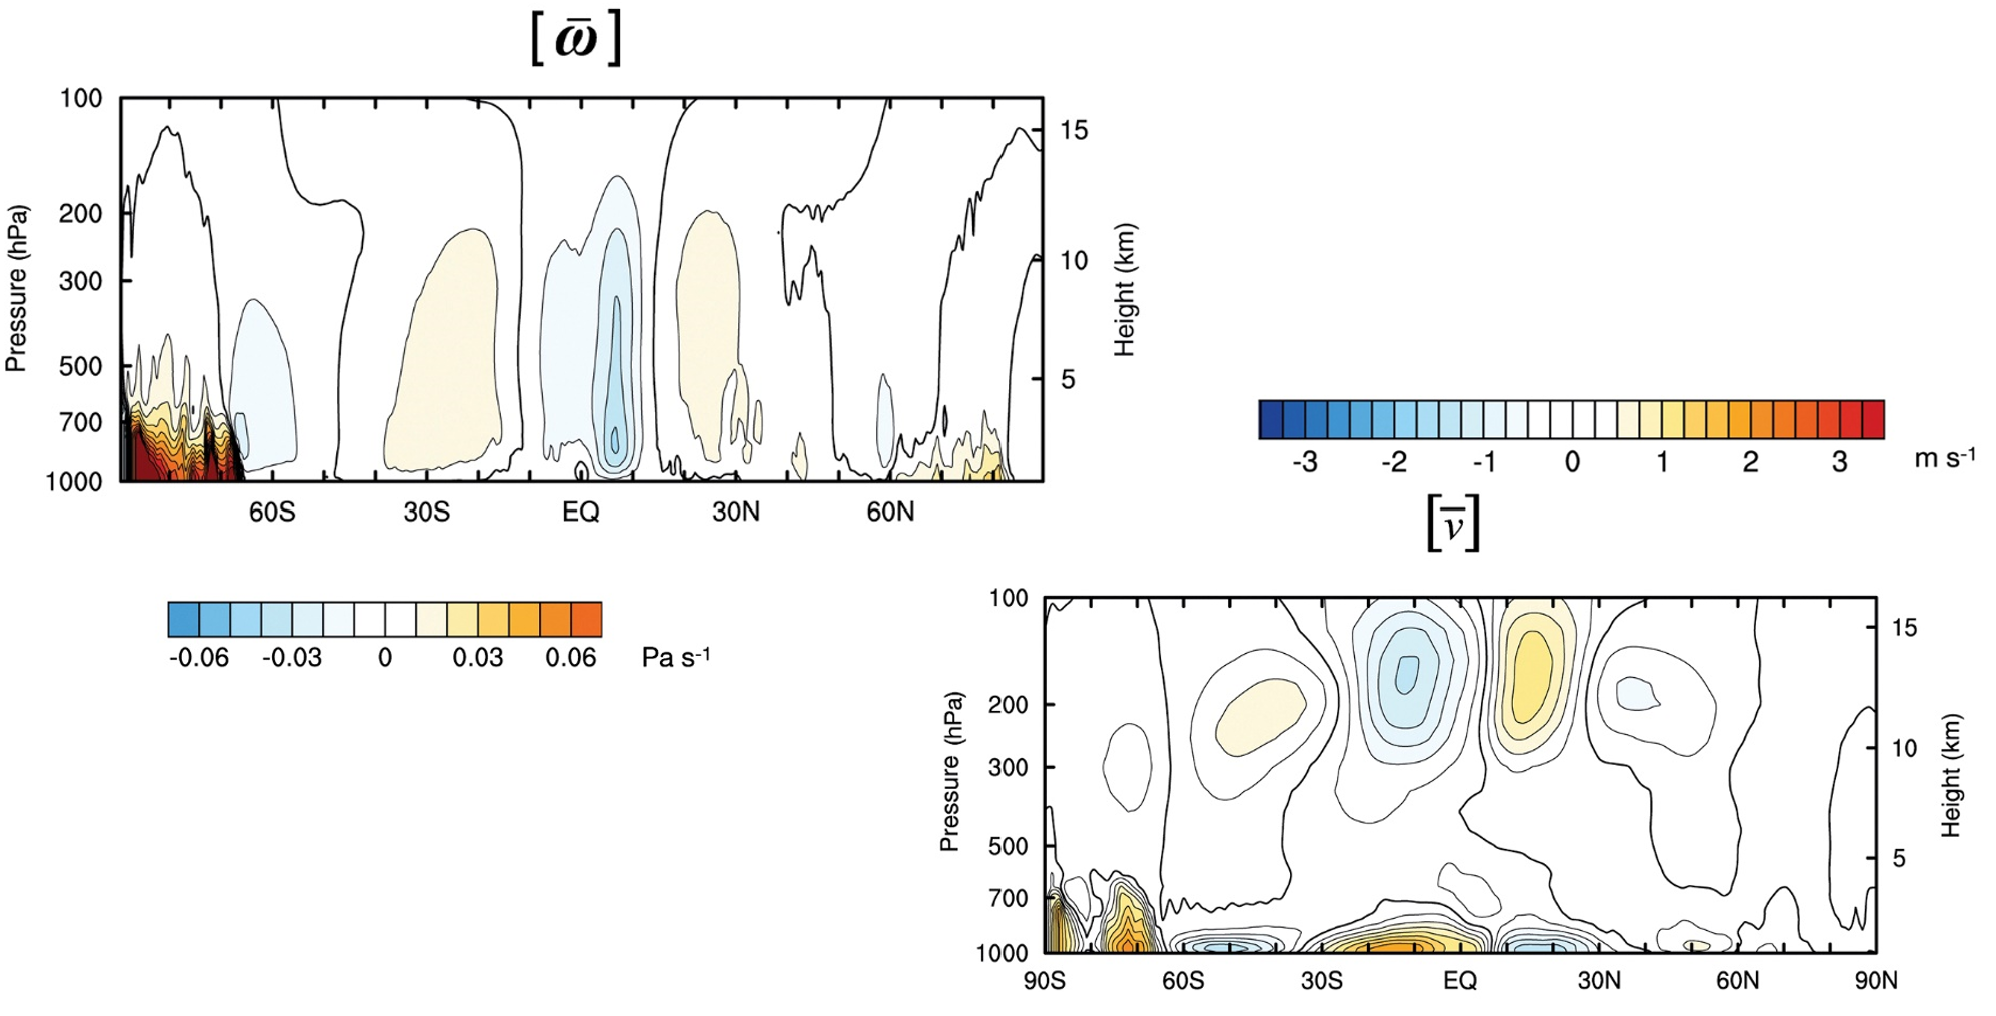
\includegraphics[width=0.5\linewidth]{uploads/mean meridional circulation.png}
    \caption{Mean meridional circulation}
    \label{fig:mean meridional circ}
\end{figure}
\subsection{Stream function}
On fig.\ref{fig:meridional streamf} lines of constant meridional stream function. In gen the flow is along lines on contant streamfunction. 
\begin{figure}
    \centering
    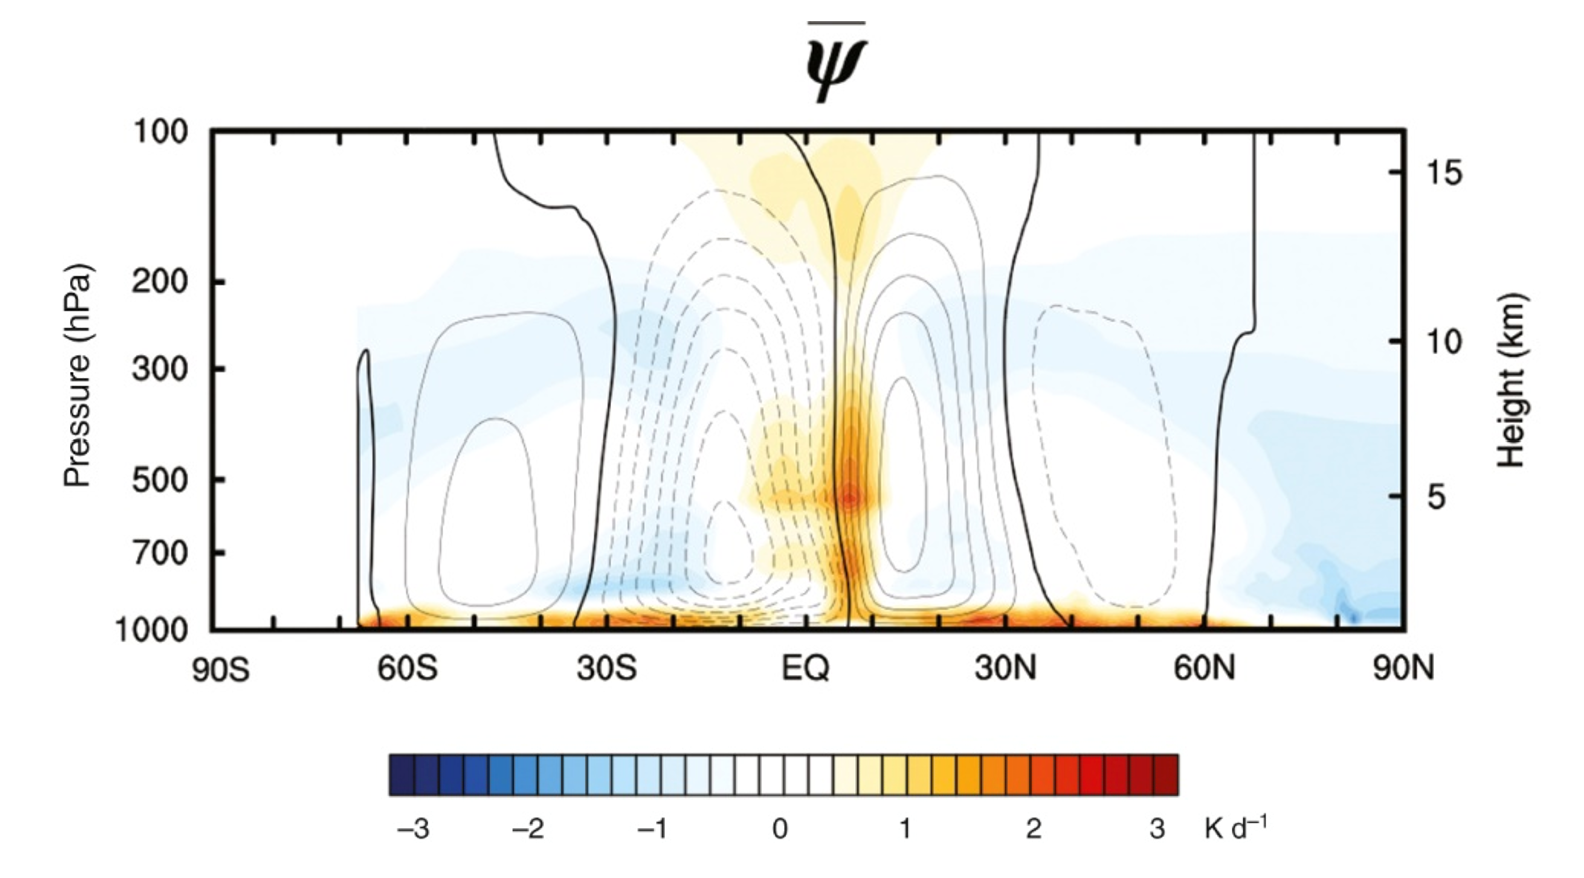
\includegraphics[width=0.5\linewidth]{uploads/streamf.png}
    \caption{Meridional mass streamfunction (contours) and diabatic heating rate (shading)}
    \label{fig:meridional streamf}
\end{figure}
A streamfunction is the best way to describe meridional mean. In general you can introduce a streamfunction in a 2D flow if the divergence of the flow is zero.
\[\text{if }\frac{\partial u}{\partial x}+\frac{\partial v}{\partial y}=0\Leftrightarrow \exists \psi(x,y)\text{ such that } u=\frac{\partial\psi}{\partial y}\quad v=\frac{\partial\psi}{\partial x}\]
note that the condition that the divergence of the flow is zero corresponds to the incompressible flow approximation. Hence, the streamfunction simplifies the flow and it gives the direction of the flow. The latter is because as $\nabla\psi\cdot(u,v)=0$ then the gradient is perpendicular to the wind, meaning that on the lines of constant $\psi$ the wind will always be perpendicular to the flow $\leftrightarrow$ the flow is always along the lines of constant $\psi$.
Notice that $\psi_0-\psi_1$ describes the mass flux of air in that region:
\[\int_{y_0}^{y_1}\rho udy=\rho\int_{y_0}^{y_1}\frac{\partial\psi}{\partial y}dy=\rho(\psi_1-\psi_0)\]
meaning that the largest $\psi$ the largest is the mass transport. In these considerations we're taking the zonal mean: we consider only 2D without the vertical component; we cannot define the streamfunction for the atmosphere but we can for the zonal mean of the atmosphere. Meridional $\psi$ is useful to describe the three cells circulation:
\[\nabla_h\cdot\vec{V}_h+\frac{\partial\omega}{\partial p}=0\] that is the continuity equation in $p$-coordinates, in spherical coordinates it can be translated into:
\[\frac{1}{R_E\cos\varphi}\left[\frac{\partial u}{\partial\lambda}\right]+\frac{1}{R_E\cos\varphi}\frac{\partial}{\partial\varphi}\left[v\cos\varphi\right]+\frac{\partial[\omega]}{\partial p}=0\]
where we took the zonal mean, recall:
\[\left[\quad\right]=\frac{1}{2\pi}\int_0^{2\pi}d\lambda\]
since $\displaystyle \frac{1}{2\pi} u\big|_0^{2\pi}=0$ (over a circle), 
\[\frac{\partial}{\partial\varphi}\cos\varphi[v]+\frac{\partial}{\partial p}\left(R_E\cos\varphi[\omega]\right)=0\Leftrightarrow \frac{\partial u}{\partial x}+\frac{\partial v}{\partial y}=0\]
so that we can introduce a streamfunction such that 
\begin{align*}
    \cos\varphi[v]=\frac{\partial\psi_M}{\partial p}\\
    R_E\cos\varphi[\omega]=-\frac{\partial\psi_M}{\partial\phi}
\end{align*}
that is called the \emph{meridional streamfunction}
\begin{equation}\label{eq.meridional streamfunction}
    \psi_M(\phi,p)=\int_{p_s}^p\cos\phi[v]dp
\end{equation}

Tropics associated with ITCZ. 
We described the mean meridional circulation with the meridional streamfunction. 
$$\psi_M(\phi,p,t)$$ formed like a 2D divergence equation. the streamfunction is useful as it defines the stream of the flow (how wide is the Hadley cell) and also the strength of the overturning. In the scientific literature to define the eedge of the Hadley cell in the middle of the troposphere (500m). You find the latitude where the $\psi_M=0$. People defined this latitude as the edge of the Hadley cell. This is important because the weather and climate in the Tropics (tropical circulation) is always below the Hadley cell. Research question: you have to find out if the Hadley cell is moving foreward: under the effect of global warming cell expands. Overturning tropical circulation is getting weaker due to global warming: you can take the different of the streamfunction: streamflow over two points: you could take the difference between the two points. The max of the Hadley cell equals the mass flow transported: how strong or weak it is. If the Hadley cell expands the Tropics get closer to the poles. Where there's the downwelling branch of the Hadley cell we have the dry zones (while upwelling we have precipitations). If the Hadley expands, the dry zones expand poleward. 
Mean meridional circulation, function of $(\phi,p,t)$ often we look it as annual mean but we can look it as seasonal mean. 
\begin{figure}
    \centering
    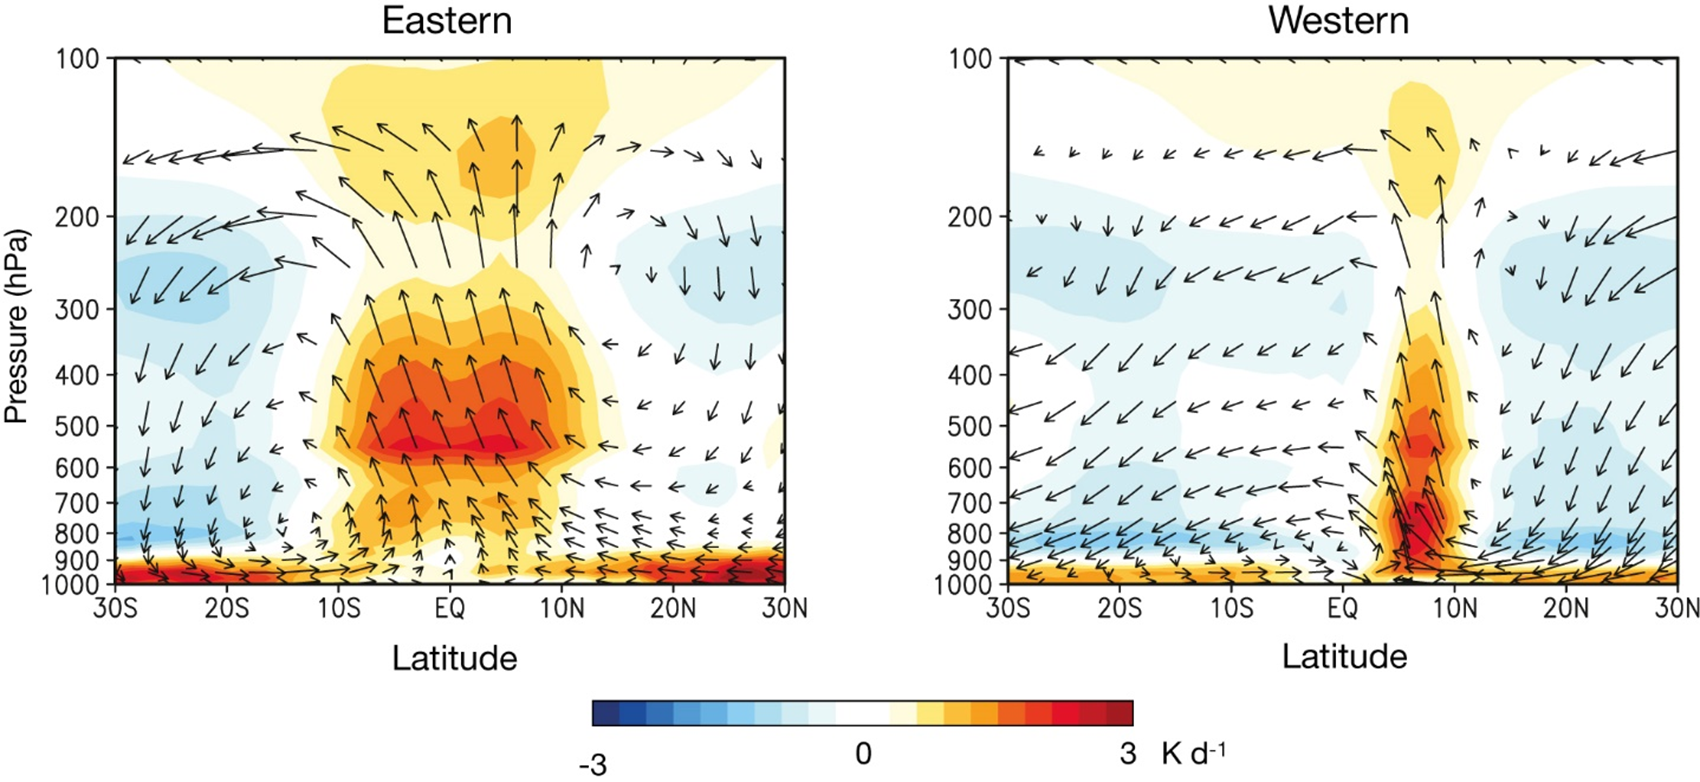
\includegraphics[width=0.5\linewidth]{uploads/winds.png}
    \caption{Enter Caption}
    \label{fig:enter-label}
\end{figure}
Longitudinally the mean meridional circulation can have different shape. The annual mean Hadley cell is quite symmetric seasonally due to larger than the other (smaller and weaker). Seasonal evolution of the Hadley cell. There's one cell much stronger that goes as uprising in the SH and upwelling in the NH. 
\begin{figure}[htpb]
    \centering
    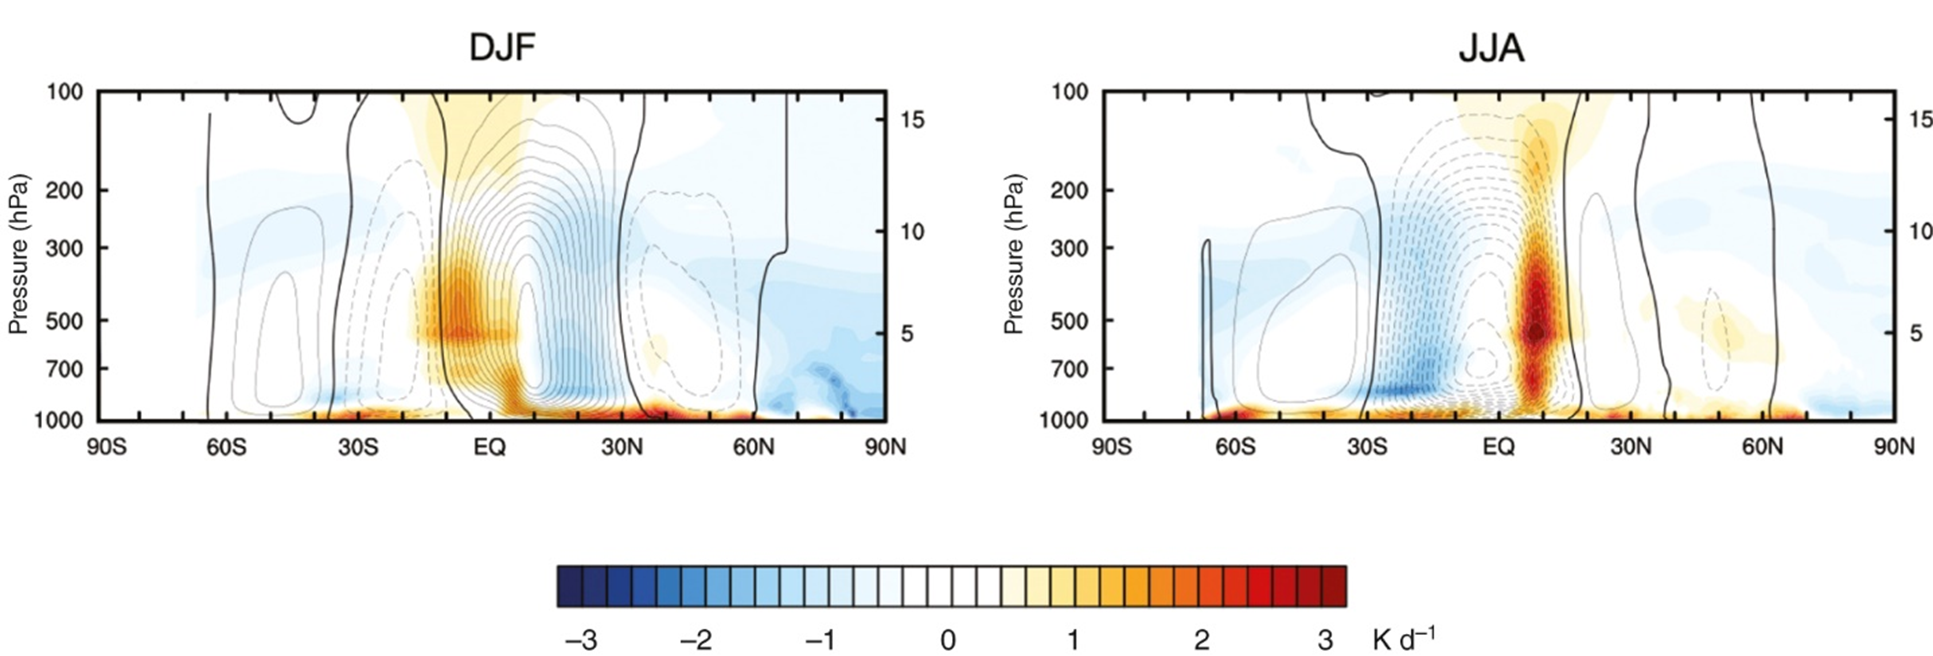
\includegraphics[width=0.5\linewidth]{uploads/meridional stream.png}
    \caption{Meridional mass stream function (contours) and diabatic heating rate (shading), seasonal variation}
    \label{fig:mass}
\end{figure}

\begin{itemize}
    \item \textbf{Winter Hadley cell} is the strongest one. It has part of it in the northen hemisphere. The upward branch is NH in the summer (rising in the winter); down-welling motion in the winters. It dominates over the two. It's the only one of the two (in fig.\ref{fig:mass}) that has a component in the Northen Hemisphere. Uprising branch always in the summer hemisphere.
    \item The weaker one has uprising and downward branch in the summer. It gets weaker and narrower.
\end{itemize}
Seasonally these two change a lot. These variations are associated with monsoons. They start when there is a strong rearragement of the Hadley cell (April, May). 
These variations are associated with monsoons in the Northen Hemisphere in summer (we have uprising and it rains) with down-welling in the other hemisphere. From 20 N to 10 S, Hadley cell shifts and the winter cell comes forward: understanding this shift is crucial to understand monsoons. 

Looking at the annual mean: the monsoons start when there's strong rearragement: FIG. ANNUAL MEAN
representing a shift northward. Mean meridional circulation is associated with monsoons, rainfalls and position of the dry zones. 


Research question: understanding how MMC changes with global warming is crucial: climate models project on expansion of Hadley cell. Wakening of the overturning meridional circulation also affects other circulation, like Walker circulation (that is East-West), where you have down-welling in the Pacific. 


Remember: condansation heats the atmosphere, while drops evaporating cools the atmosphere. Fig.\ref{fig:mass} shows that a large amout of heat is release because there's condensation. Because of convection the atmosphere is heated due to thunderstorms. Where the atmosphere is cold there's emission of IR radiation. You can conclude that the atmosphere is heated up in the middle of the troposphere and tropical rainfalls where you have monsoons in tropical convergence zone and near the surface (fluxes of sensitive heat and latent heat) CHECK BOOK.


How do we identify where the transient acts? There are pars of the world where circulation is zero. If we look at a single day you see a different structure evolving that has both vertical and meridional component $\leftrightarrow \quad \bar{v}=0 \quad v'\neq 0$. We can look at the variance $\overline{v'^2}$ or the standard deviation $\sigma (v')=\sqrt{\overline{v'^2}}$ that can be different from zero even in the case of $\overline{v'}=0$. This is a good proxy to identify where the transient is acting and how strong. 

Time mean of geopotential height sigma figure. $\sigma (v'_{200})$ meridional wind at $200$ hPa in a single day: there are two regions in the extra tropics where it is higher: stormtracks. At tropics circulation is more stable in time (a lot of transients = very large $\sigma\rightarrow v'\neq 0$). 

\begin{figure}
    \centering
    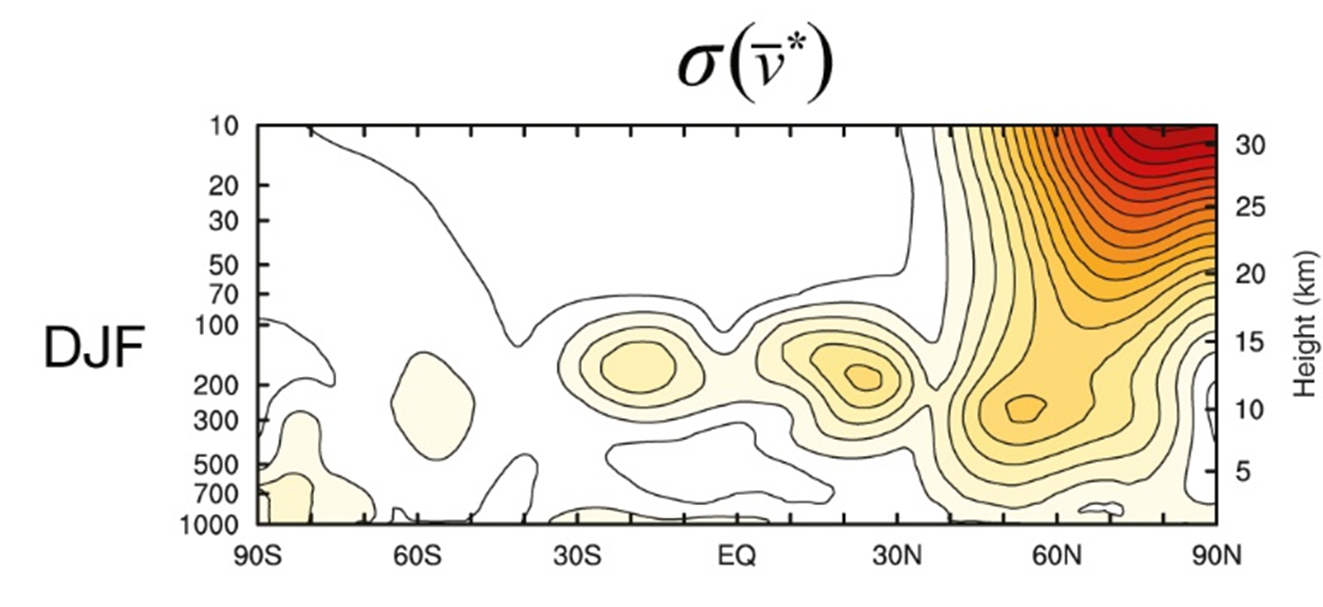
\includegraphics[width=0.5\linewidth]{uploads/sigma vmean.png}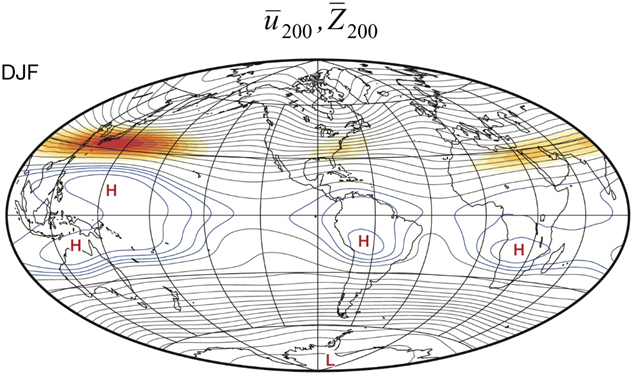
\includegraphics[width=0.5\linewidth]{uploads/sigma vmean world.png}
    \caption{$\sigma(\bar{v})$}
    \label{fig:sigma vmean}
\end{figure}
\begin{figure}[htpb]
    \centering
    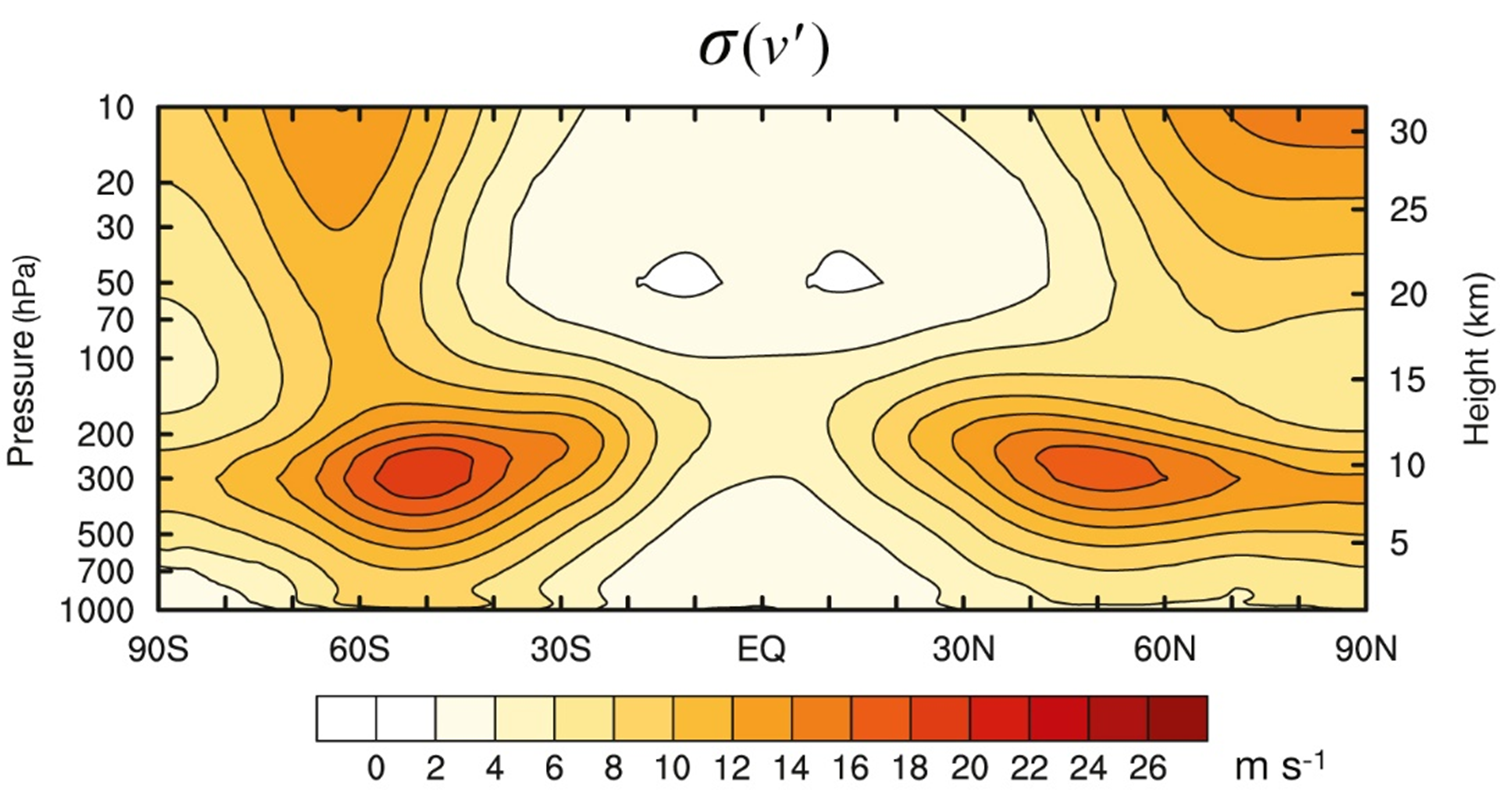
\includegraphics[width=0.5\linewidth]{uploads/sigma vtrans.png}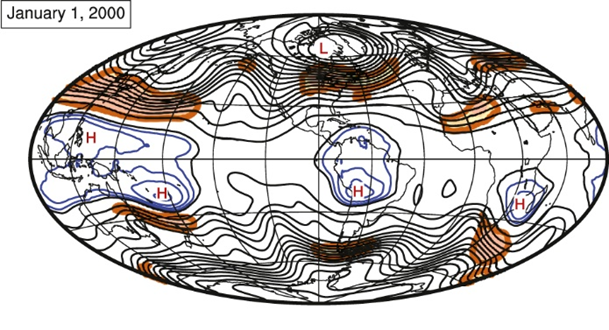
\includegraphics[width=0.5\linewidth]{uploads/sigma vtrans world.png}
    \caption{$\sigma(v')$}
    \label{fig:sigma vtrans}
\end{figure}

Remember: if I have a through there will be a cyclone developing under it.

For each single day you can work out the deviation and square time mean and variance up to 200 hPa: there are two regions on the extra tropics where the variance is larger: they corresponds to storm tracks. Circulation in the tropics is much more stable. These waves that form and moves around mean a lot of transient, reflected in veri large standard deviation in the mean meridional wind almost close to zero (isobars are almost symmetric). 
\begin{figure}[htpb]
    \centering
    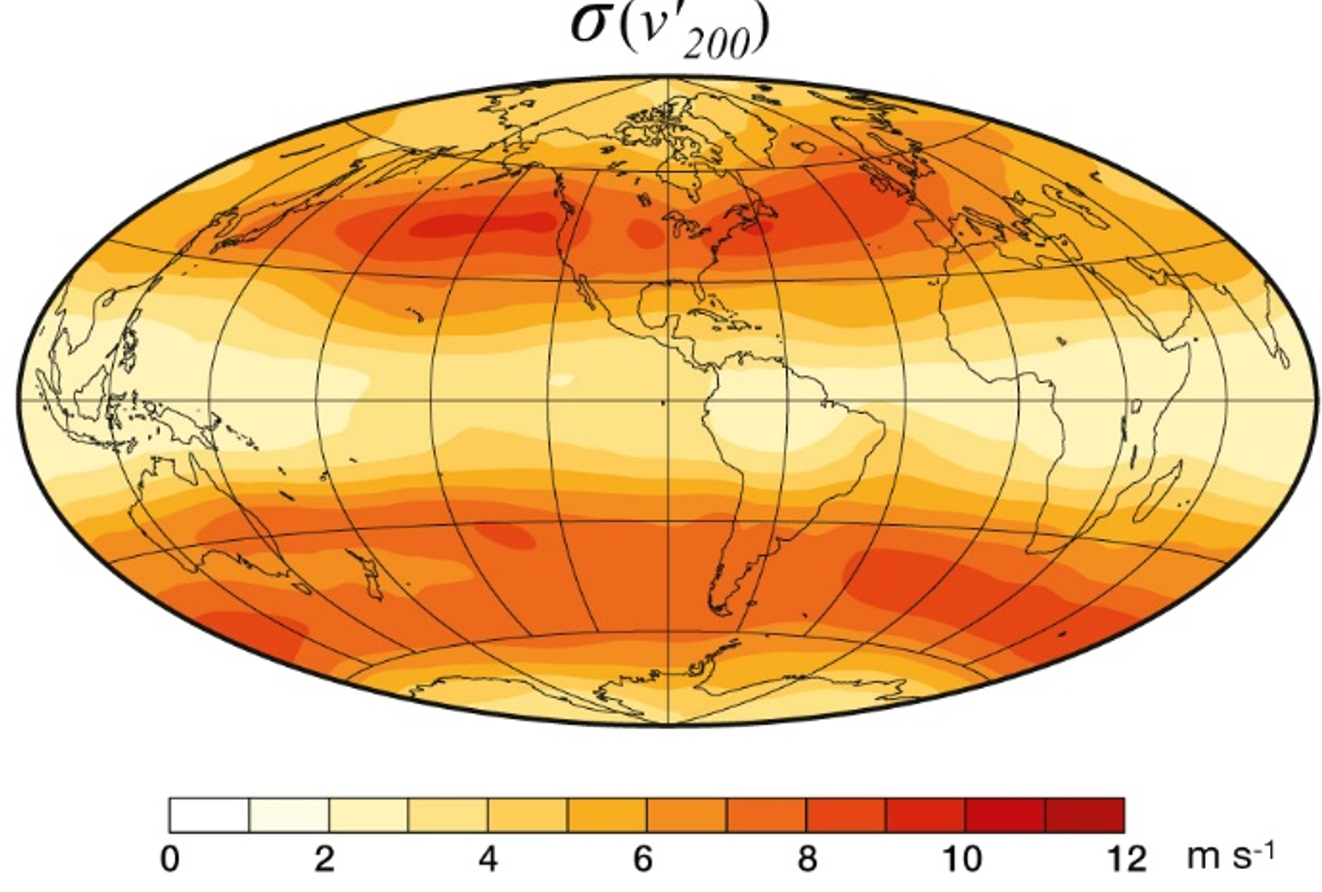
\includegraphics[width=0.5\linewidth]{uploads/sigma v(200).png}
    \caption{$\sigma(v'_{200})$}
    \label{fig:sigma v'}
\end{figure}
Research question: how storm tracks change under global warming. Climate models suggestions show that extra tropical storm tracks will shift poleward with global warming. How do people identify this? Working out standard deviation of meridional wind, you can also other values such as vertical wind: that's a quantity that if you average over time in extra tropics goes to zero. Days with high pressure vertical wind is downward, when cyclone (rains) by def you have upward. When you are in a region with both high and low pressure the average goes to zero, you can use the std dev of $\omega$. One of the best proxies to identify when it rains (fig.\ref{fig:sigma and precipit}). Rain forms in the few km. Transient in the vertical best capture what happens during tropical cyclone. $\sigma(w'_{700})$ is the verticl velocity at $700$ hPa $\sim 3$ km above the surface where condensation happens. In this figure we clearly see N.Atlantic and N.Pacific storm track. 
\begin{itemize}
    \item $\overline{w}_{500}$ mean time vertical velocity correlates well with rain but we don't see the transient. 
    \item At high latitudes rain is associated with transients. 
\end{itemize}
Who studies monsoons focuses on mean flow whereas who studies transients focuses on the variation of the mean flow. 
\begin{figure}[htpb]
    \centering
    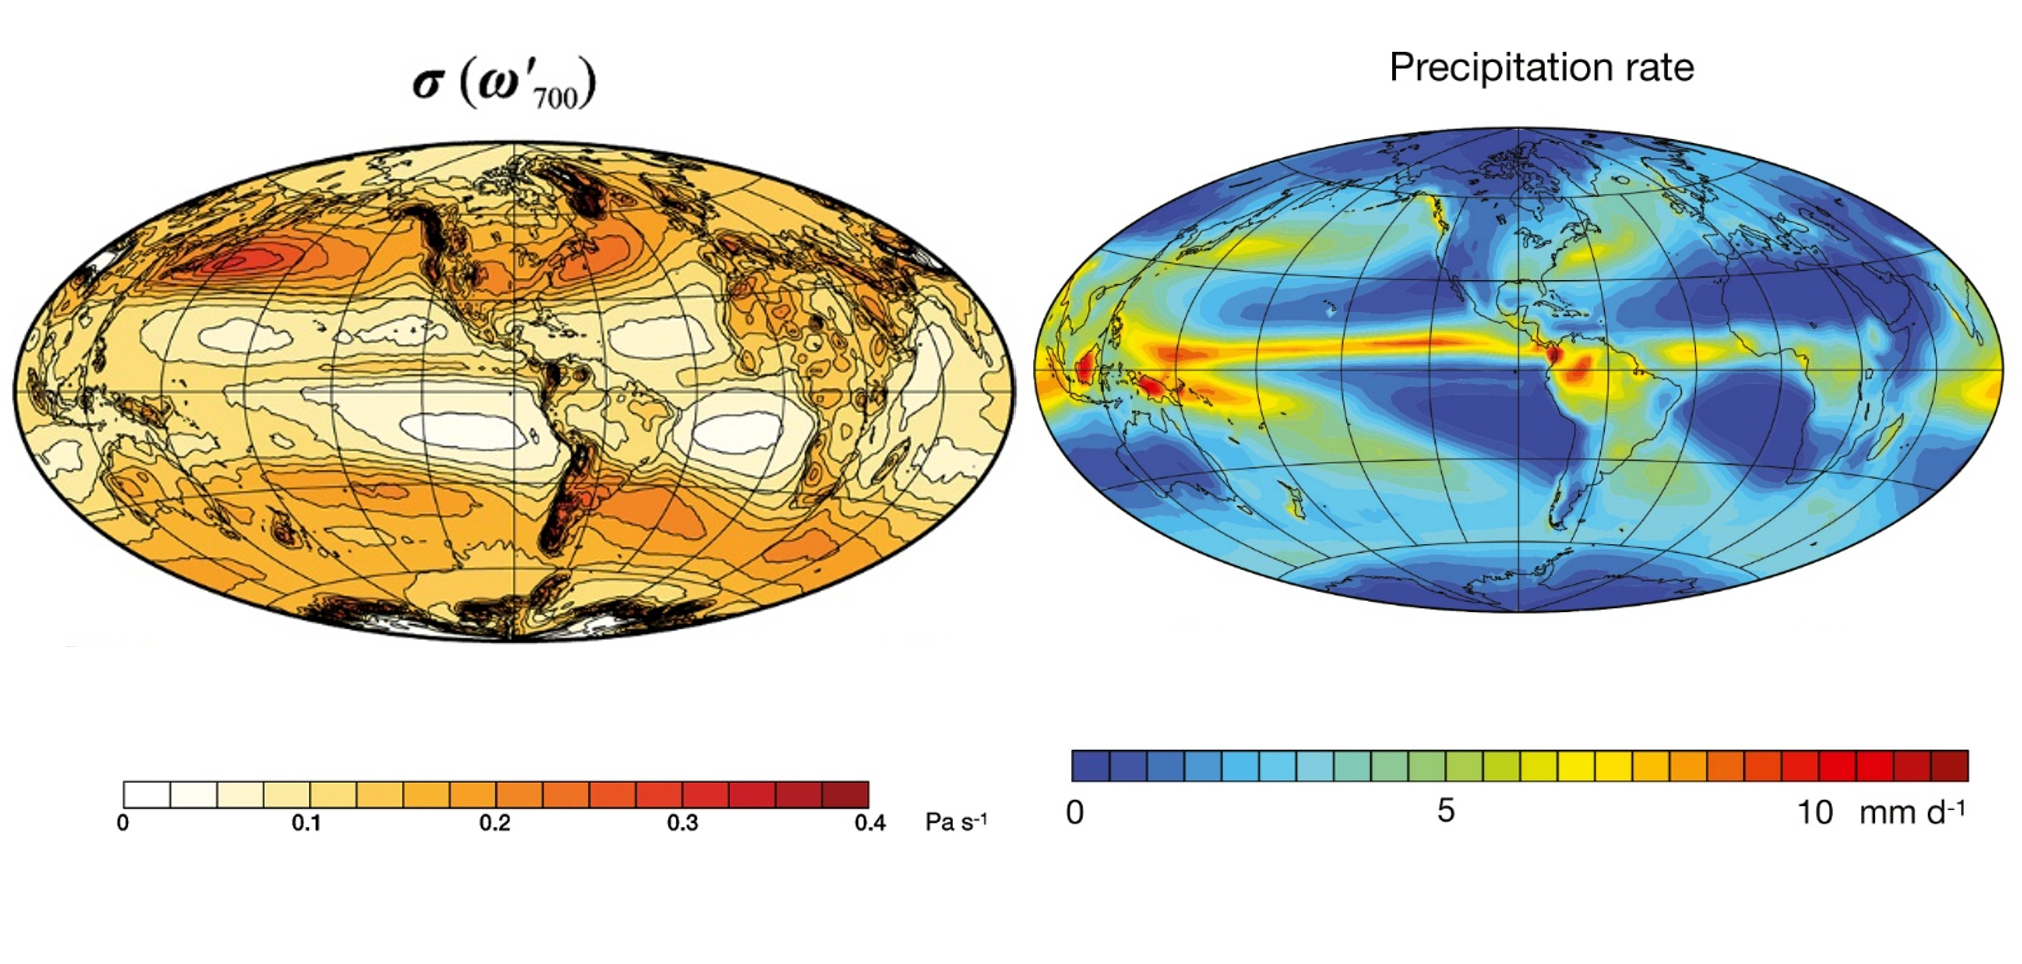
\includegraphics[width=0.5\linewidth]{uploads/sigma and precipitation.png}
    \caption{Correlation between sigma and precipitations}
    \label{fig:sigma and precipit}
\end{figure}
\begin{figure}[htpb]
    \centering
    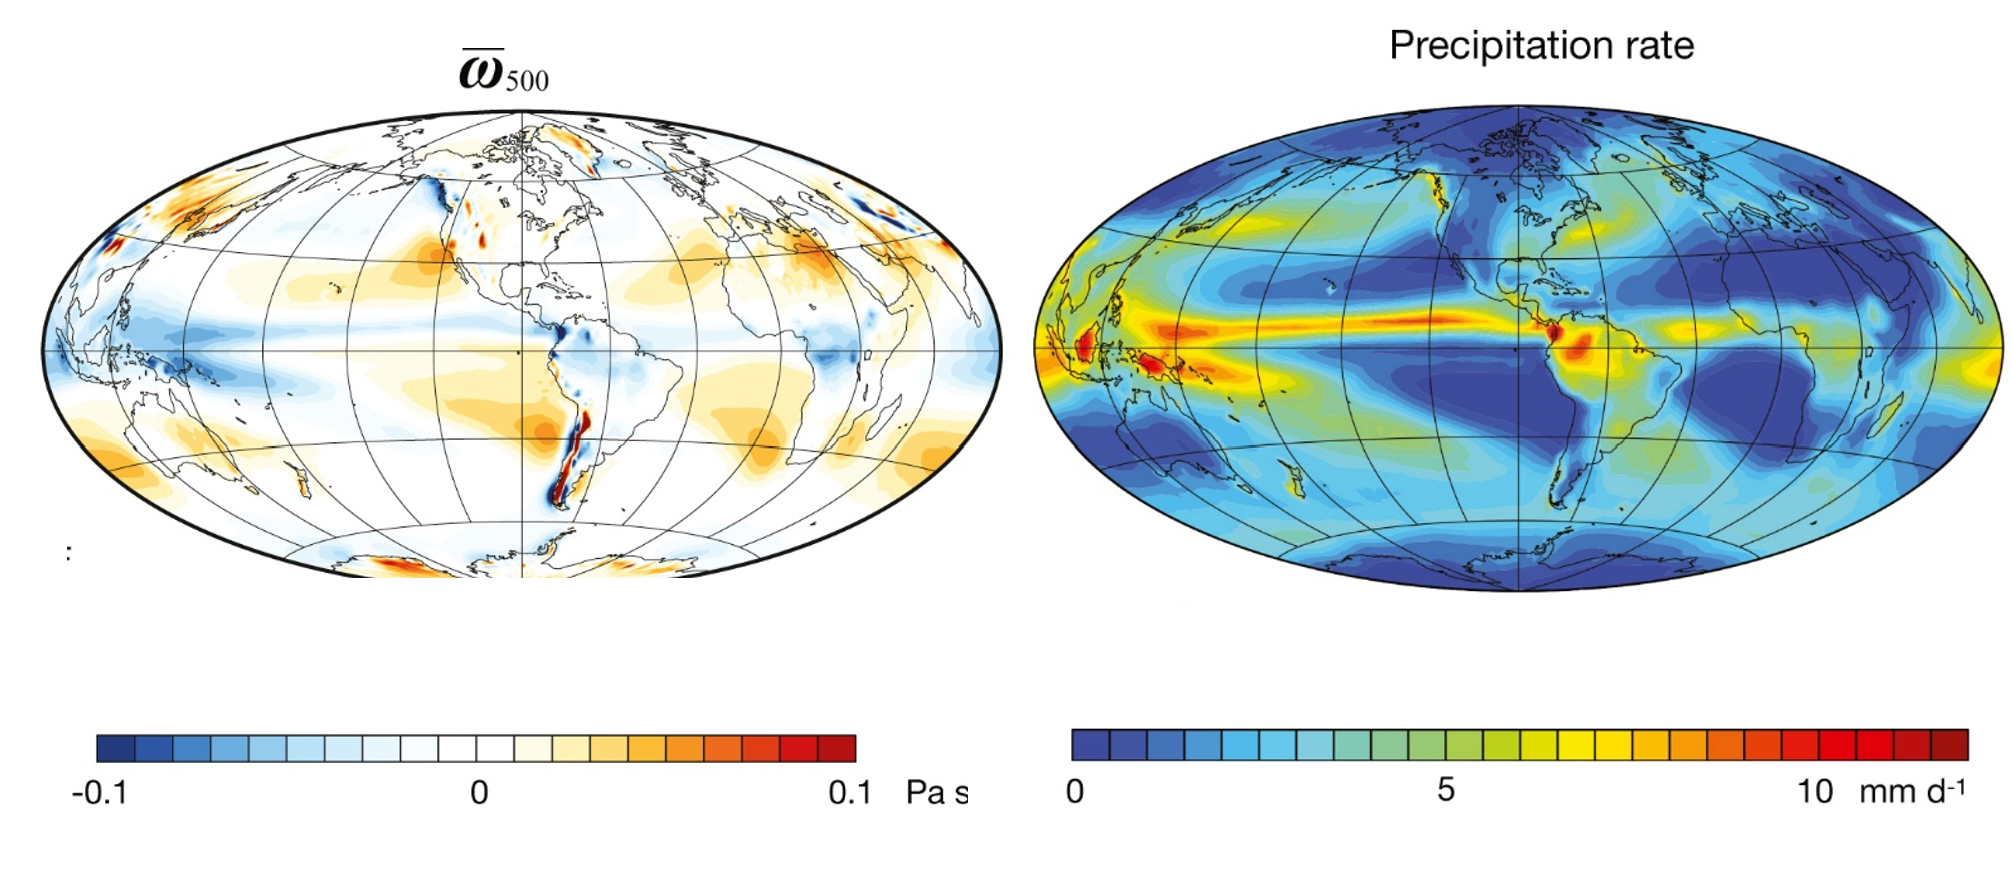
\includegraphics[width=0.5\linewidth]{uploads/omega and precipit.png}
    \caption{Correlation between $\omega$ and precipitation}
    \label{fig:omega and precipit}
\end{figure}



If you look at the mean precipitation you see that the spatial distribution of the vert velocity correlates well with the structure of precipitation but it doesn't for ITCZ: rains at high lat are not associated with mean circulation but with transients: when it rains in high lat is because you have a cyclone, it doesn't rain bc there's high pressure. 

When we looked at the mean vert velocity: this field correlates with tropical rainfall but it doesn't show storm tracks. You can conclude that tropical rainfall in the ITCZ or monsoons are mostly associated with mean meridional circulation (very nice correlation) and Hadley cells, whereas precipitations in the extra tropics (storm track region) nota associated with the mean circulation, but you see it in the transients (rain in the extra tropic is not associated with persistent phenomena but with transients). 




\section{The water cycle}
Transport influenced by the atmospheric general circulation. Evaporation (or evapotranspiration) is a source and precipitation is a sink. Surface runoff (rivers and channel) or underground runoff (groundwater). Atmospheric branch and land branch of the water cycle connected by processes of precipitation and evaporation. Atmosphere contains only 0.001\% of water: it's the smaller reservoir but the most dynamic in terms of transferring water from one place to another.
\begin{figure}[htpb]
    \centering
    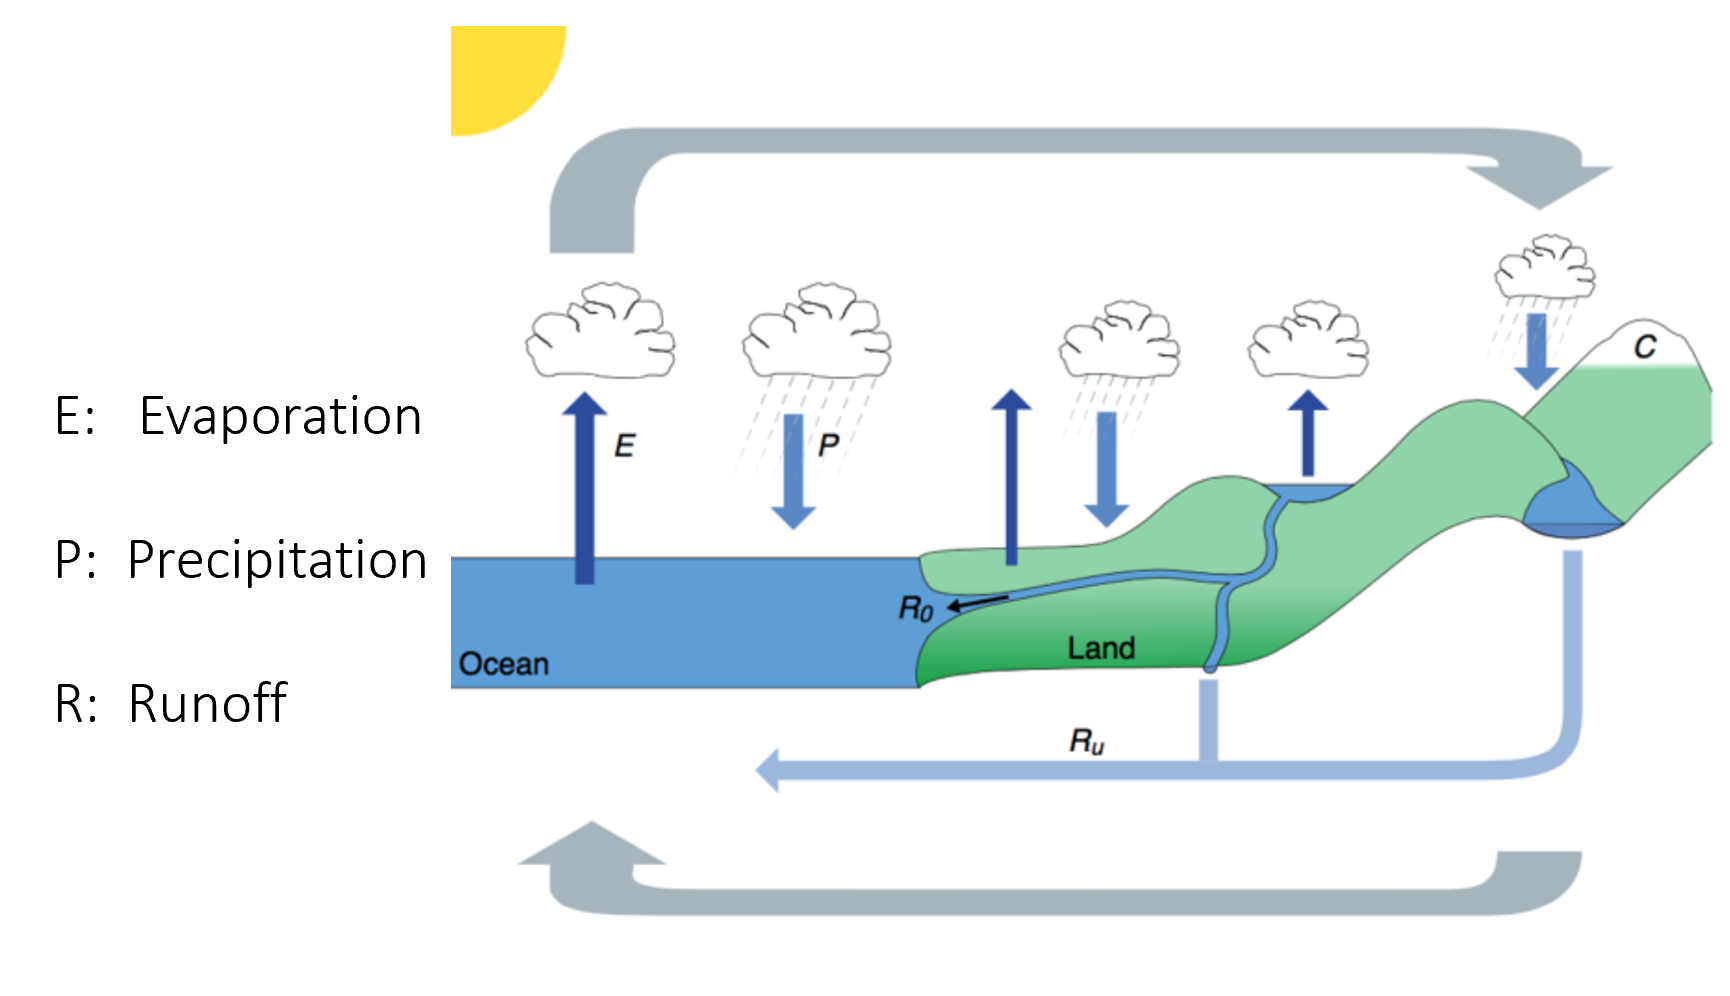
\includegraphics[width=0.5\linewidth]{uploads/water cycle.png}
\end{figure}
\begin{figure}[htpb]
    \centering
    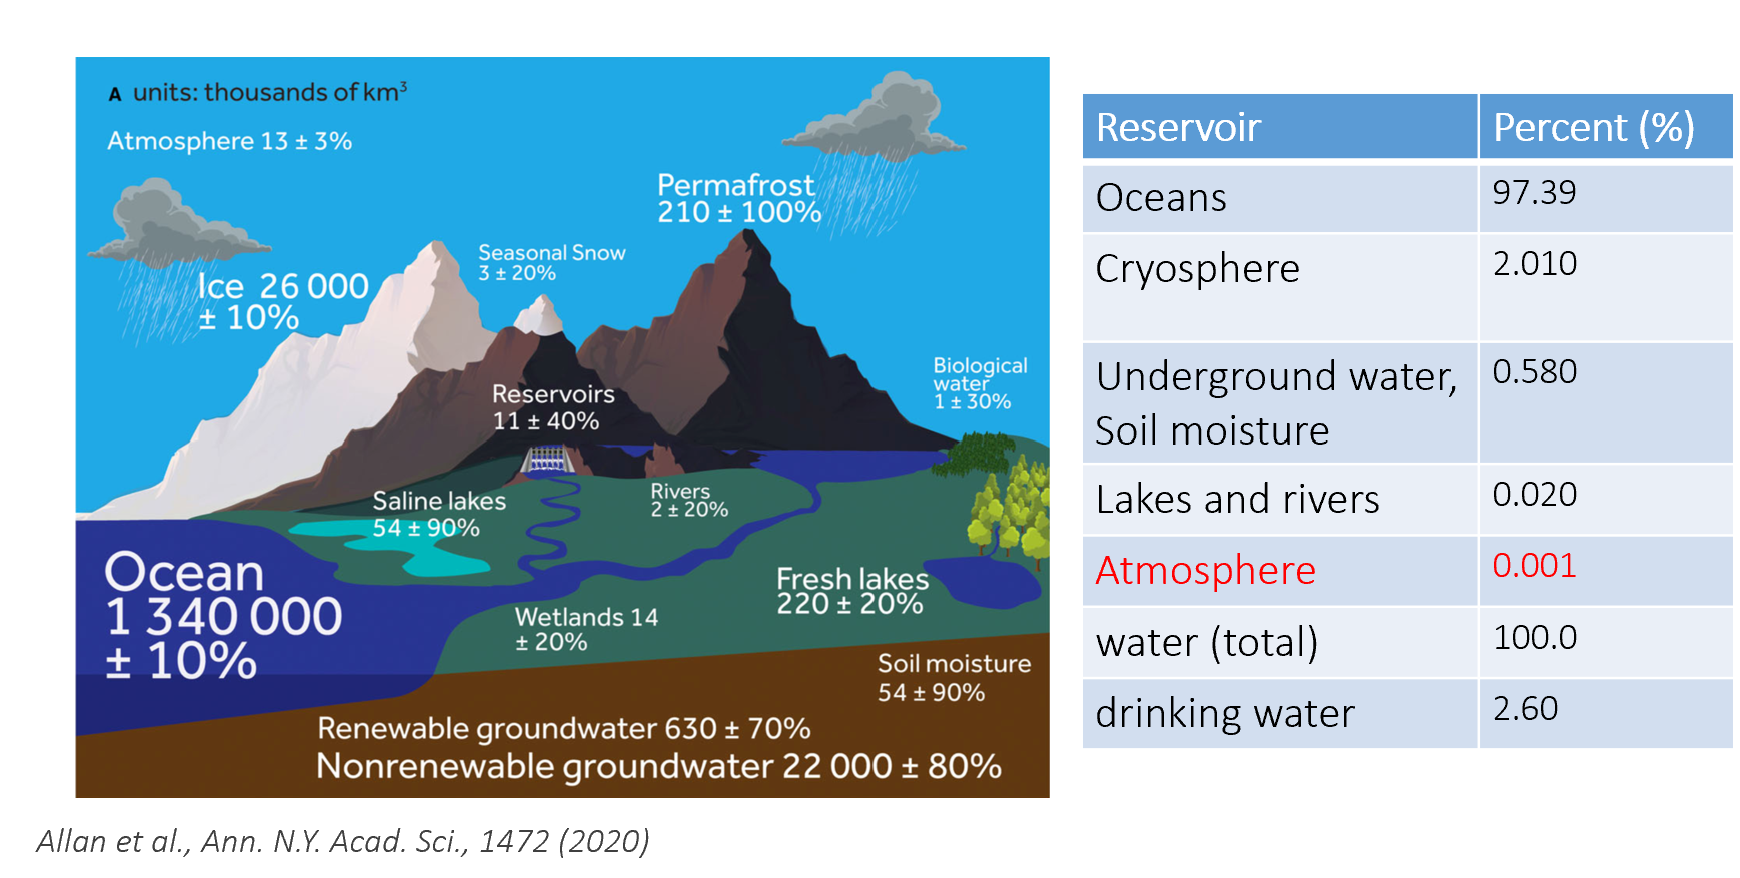
\includegraphics[width=0.5\linewidth]{uploads/water content.png}
\end{figure}
Atmosphere is moving water vapor around: the fluxes related to it are big.
\begin{figure}[htpb]
    \centering
    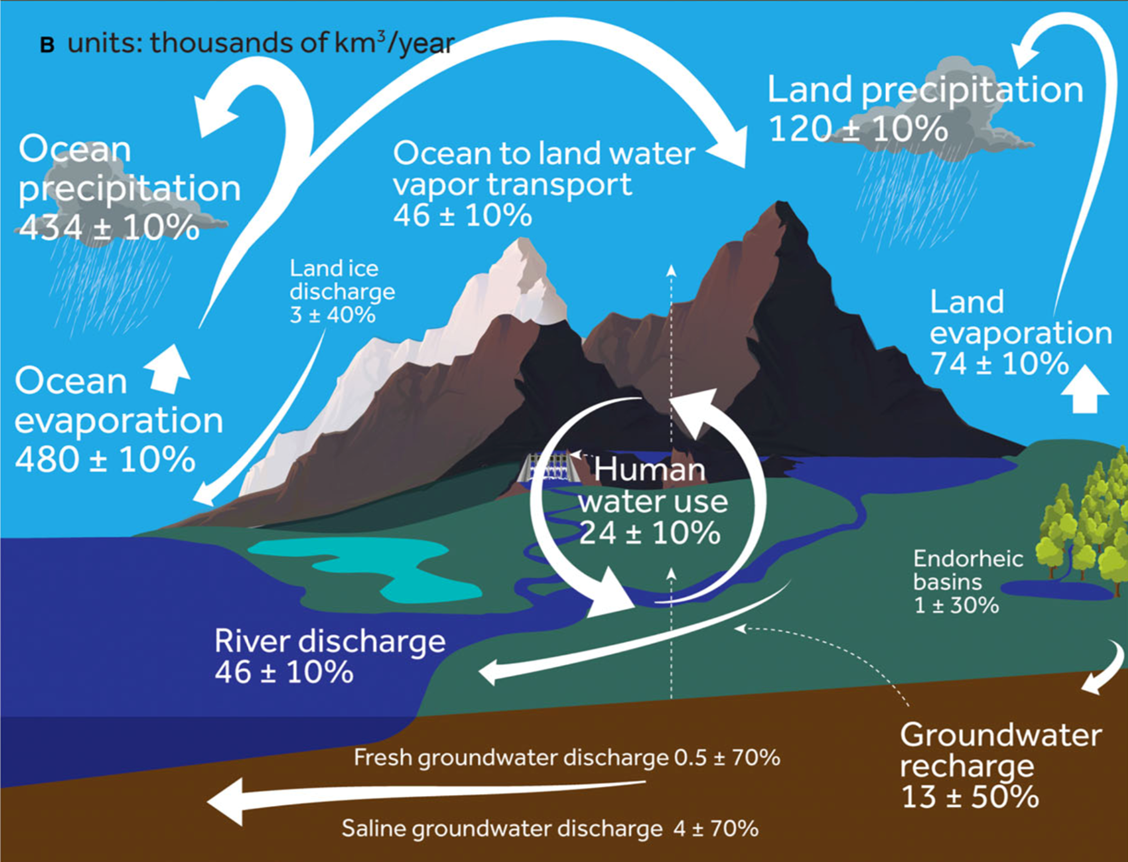
\includegraphics[width=0.5\linewidth]{uploads/water fluxes.png}
    \caption{Water fluxes}
    \label{fig:water fluxes}
\end{figure}
Important variables:
\[\text{specific humidity: }\quad q \quad [\text{g/kg}]\]
\begin{figure}[htpb]
    \centering
    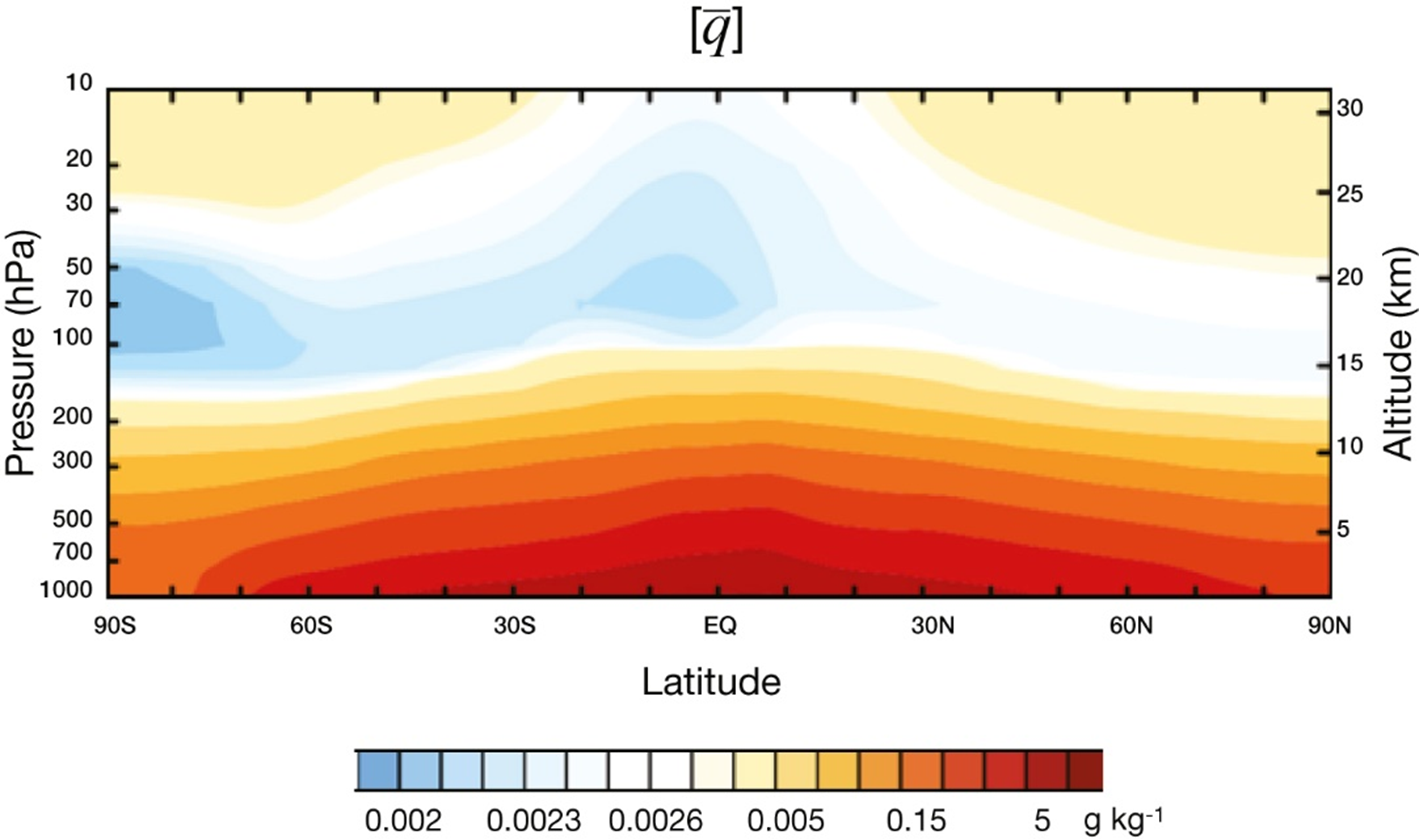
\includegraphics[width=0.5\linewidth]{uploads/specific humidity.png}
    \caption{Specific humidity: concentration of water vapor in the atmosphere.}
    \label{fig:q}
\end{figure}
Mostly concentrated in the few km of the atmosphere and it's higher is in the Tropic: the warmer atmosphere, the more water vapor it can contain. Clouds are made of droplets or ice in the pole. Water is also contained in clouds: $q+q_l+q_i$ specific concentration of water vapor, liquid water and solid water, we will just consider $q$: we can do it because the gas component accounts for most of all water in the atmosphere. 
Clouds contain either $q_l$ or $q_i$, if you consider $\displaystyle\frac{\text{mass of clouds}}{\text{mass of all water on the atmosphere}}=\frac{1}{300}$
clouds are important for radiative balance but in terms of mass of water that they contain they are very negligible.
\paragraph{Precipitable water/total column water vapor (TCWV)} is just the vertical mass integral of $q$:
\begin{equation}
    W=\int_{p_s}^{0}-\frac{dp}{g}q\quad\text{kg/m}^2
\end{equation}
it says how much water vapor you have inside an atmospheric column of section $1\text{ m}^2$, it gives an indication locally on how much water vapor you have (and could be precipitation, usually it precipitates less).
\begin{figure}[htpb]
    \centering
    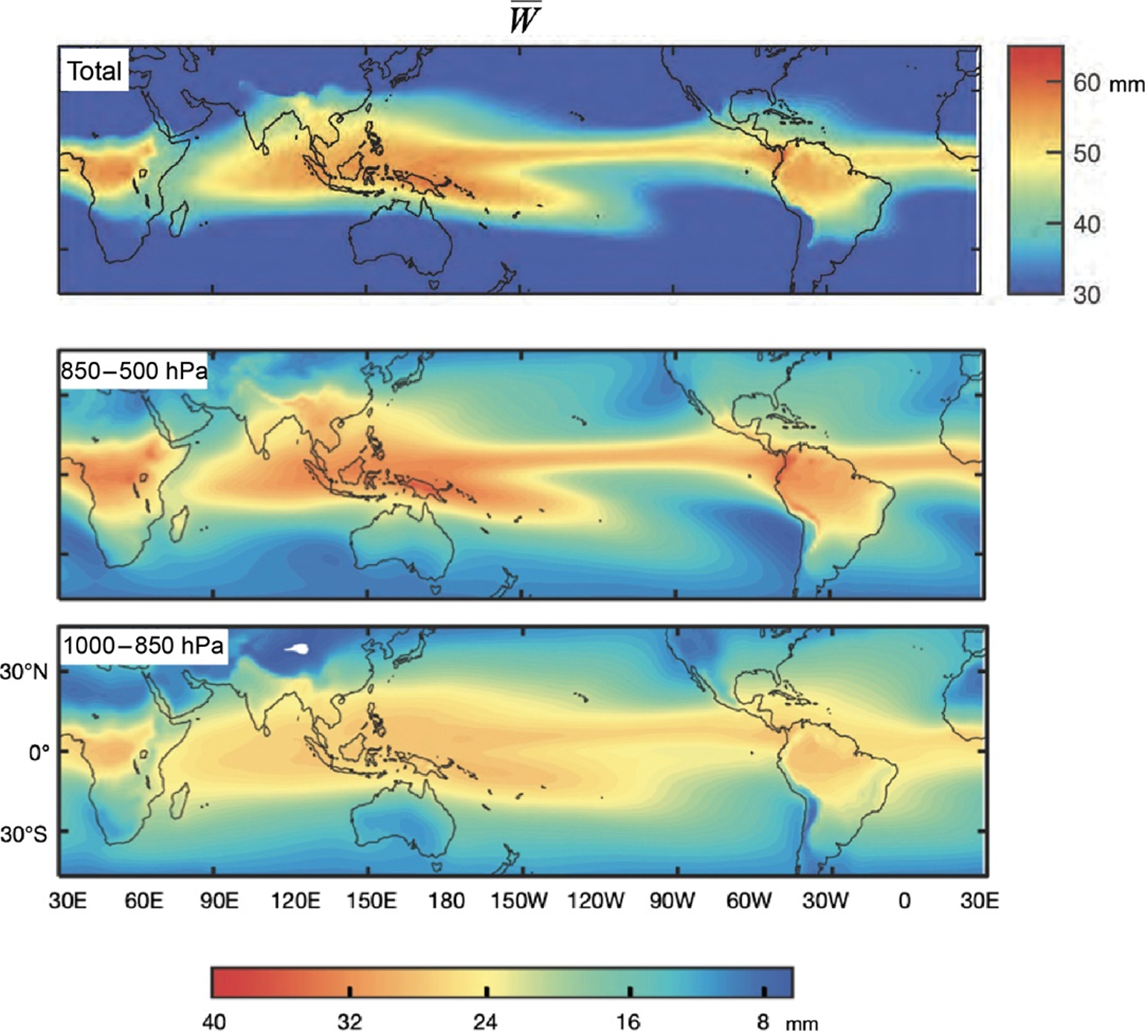
\includegraphics[width=0.5\linewidth]{uploads/W.png}
    \caption{Most of the water in atmosphere is concentrated in the Tropics}
    \label{fig:W}
\end{figure}
\paragraph{Vertically integrated vapor flux (IVF)} A water vapor flux is defined as the movement of water vapor carried by the wind: $q\mathbf{v}=(qu,qv,qw)$ specific humidity times the wind, in general it is a 3D quantity: how water vapor is transferred zonally, meridionally and vertically. The IVF is:
\begin{equation}
    \text{IVF}=\int_{p_s}^0-\frac{dp}{g}q\mathbf{v}
\end{equation}
that is a 2D quantity, meaning that the amount of water vapor transported is moved horizontally through the atmosphere. You integrate over the vertical: we're interested in what happens horizontally.
\begin{figure}[htpb]
    \centering
    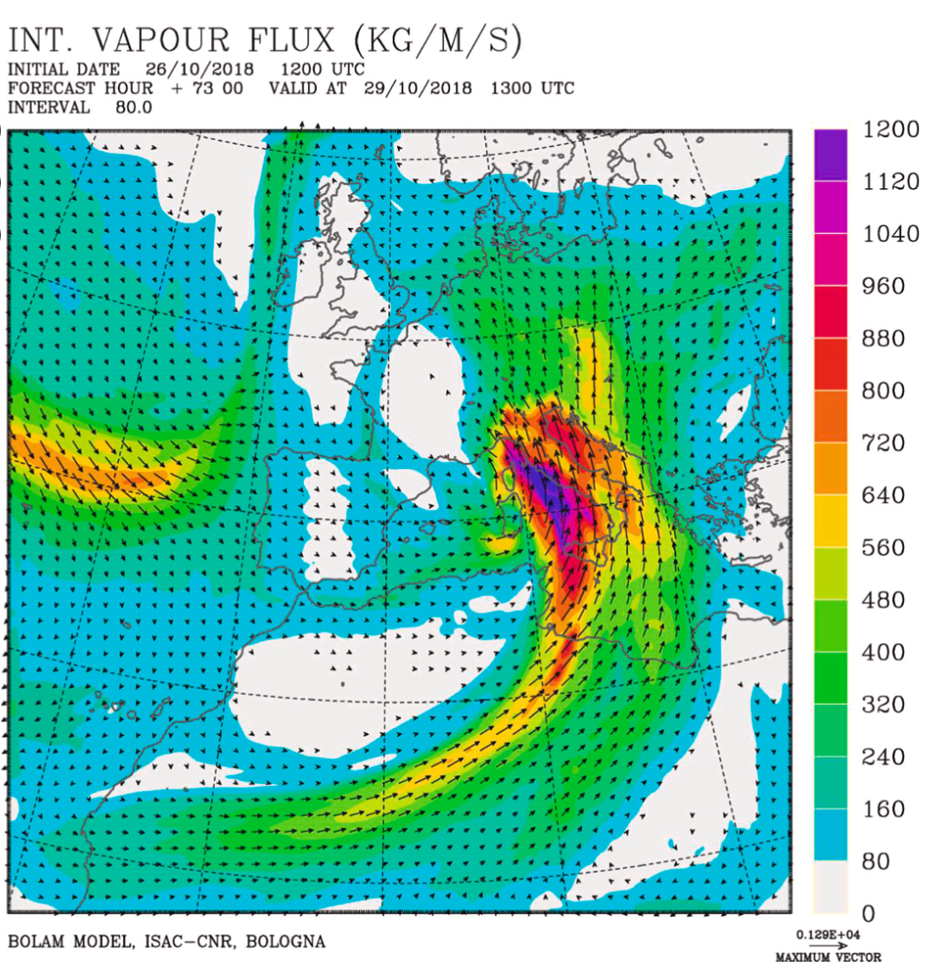
\includegraphics[width=0.5\linewidth]{uploads/VAIA.png}
    \caption{IWVF during Vaia’s high precipitation event }
    \label{fig:VAIA}
\end{figure}
In fig.\ref{fig:VAIA} Vaia was a strorm in extra tropical cyclone: strong wind and large precipitation. The arrows show the IWVF, where you have a lot of water vapor in the atmosphere, there was a river of water vapor transported over the Atlantic converging. The atmospheric circulation on that day was so that a lot of water vapor was transported. IWVP is a very important diagnostic tool for weather forecasting. \textit{Atmospheric rivers} are large transport of water vapor from the Tropics to the extra tropics, they stretch seen as interactions between extra tropical ?? they typically impact the West Coast of USA. 

In order to see where it's raining, you take the divergence $\nabla\cdot (\text{IVF})$ because divergence tells you where you have a sink or a source: negative value means it's raining. In situations in where the flow is converging somewhat, the inside area will have a negative divergence (convergence); while positive divergence is what divergence literally means. When you take IVF, you work out the divergence: piling up water vapor, it cannot disappear due to conservation of mass: you'll have large precipitation.
Also, where the field is decreasing you'll have a convergence (negative derivative) you bring in more than you bring out. In a 3D field, divergence of the hor component where it's negative upwelling, positive down-welling, in this case we integrated over the vertical hence it's a 2D field, the only way to get away is by rain.
\begin{figure}[htpb]
    \centering
    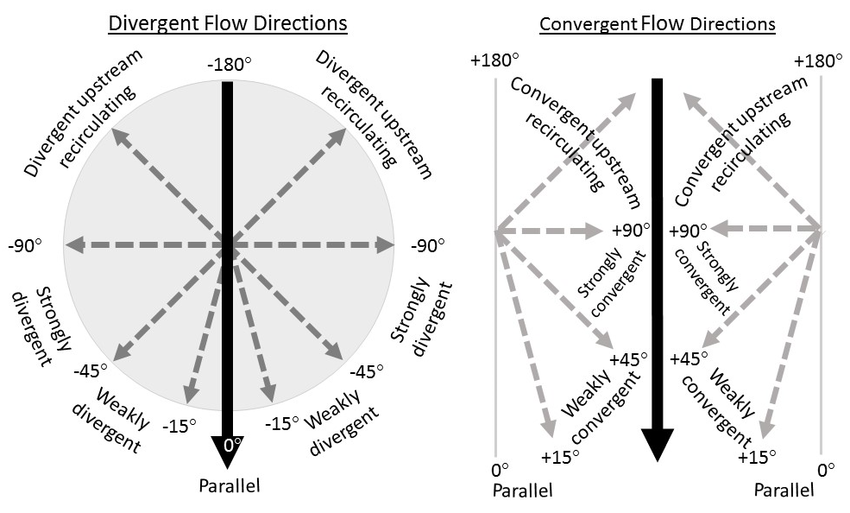
\includegraphics[width=0.5\linewidth]{uploads/divergence.png}
    \caption{Convergence and divergence}
    \label{fig:conv}
\end{figure}
\begin{figure}[htpb]
    \centering
    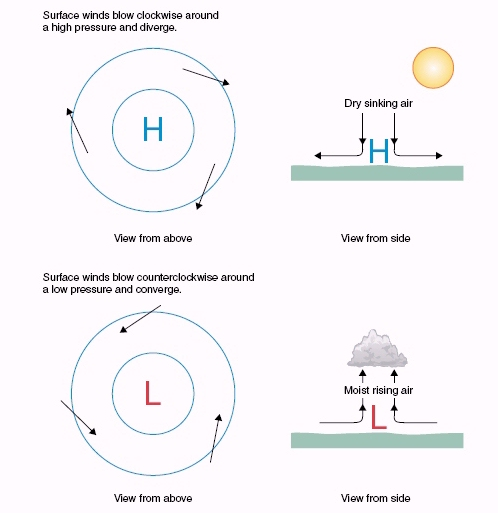
\includegraphics[width=0.5\linewidth]{uploads/convergence recall.png}
    \caption{Convergence recall}
\end{figure}

$$W=\int_{p_s}^0-\frac{dp}{g}q$$ water vapor in the atmosphere.
Vertical integrated water vapor flux: 
$$\mathbf{Q}=\int_{ps}^0-\frac{dp}{g}d\mathbf{v}$$ how water vapor is moving overall

$P$ how much water is going out from the atmosphere, water is like a sink for the atmosphere: when it rains atm is losing water vapor
$E$ evapo-transiparion (over land evapor- as it's mediated by land). I is a source of water vapor for the atmposphere. 

We will demostrate balance equation for the vertical integrated water vapor balance eq in the atmosphere
\begin{equation}\label{eq.W}
    \frac{\partial W}{\partial t}+\nabla_h\cdot \mathbf{Q}=E-P
\end{equation}
where the divergence is a 2D divergence. The time derivative f the tot amount of water vapor in the water column is give by three terms: 
\[\frac{\partial W}{\partial t}=\underbrace{(E-P)}_{\text{sources/sinks}}\underbrace{-\nabla_h\cdot \mathbf{Q}}_{\text{transport of $q$ associated with $\mathbf{v}$}}\]
differential eq: everything is true at any point.\\




You may now understand why $E$ is a source and $P$ is a sink. The sign of divergence depends on the specific vertically integrated water vapor flux. In general, when 
\begin{itemize}
    \item $\div{F}>0$ it means something is leaving my field
    \item $\div{F}<0$ you have convergence to my field.
\end{itemize}
applying this principle to $Q$, in the hor plane, regions where the hor divergence of $Q$ is positive, the flow ($Q$ is associated with $v$) tends to carry water vapor away to certain regions. Carrying water vapor away you're emptying that region: contributing negatively in the balance: decreasing water vapor in that colum. Whereas, converging water vapor in a specific regio, in the balance it contributes positively: increase of water vapor in a given column in time. $W$ can change in time either bc locally it's raining ($P$) or evaporation ($E$) or bc the flow is carrying water vapor in or out. \\


Let's consider a finite region $\mathcal{S}$ (instead of infinitesimal point) and we integrate over that region. $\partial\mathcal{S}$ defines the border of the region:
\[\int_{\mathcal{S}}\frac{\partial W}{\partial t}=-\int_{\mathcal{S}}\nabla_h\cdot\mathbf{Q}d\mathcal{S}+\int_{\mathcal{S}}(E-P)d\mathcal{S}\]
\[\frac{\partial}{\partial t}\int_{\mathcal{S}}Wd\mathcal{S}=-\int_{\mathcal{S}}\nabla_h\cdot\mathbf{Q}d\mathcal{S}+\int_{\mathcal{S}}(E-P)d\mathcal{S}\]
because the region doesn't vary in time

the first one is the time derivative of the total amount of water vapor in that region ($W$ is define per meter squared). The last term is just what's the tot amount of evaporation from land or ocean into that region and the amount of precipitation. 
Let's analyze the meaning of 
\[-\int_{\mathcal{S}}\nabla_h\cdot\mathbf{Q}d\mathcal{S}\]
using Gauss theorem (from a 2D integral to a 1D integral):
\begin{equation}\label{eq.Gauss theorem}
    \int\int_{\mathcal{S}}\div{\mathcal{Q}}\mathcal{S}=\oint_{\mathcal{S}} \mathcal{Q}\cdot \hat{n}dl
\end{equation}
Int od divergence is equal to the flux. The scalar product gives how much goes out ($Q$ and $\hat{n}$ are in the same direction or not). Hence, 
\[\frac{\partial}{\partial t}\int_{\mathcal{S}}Wd\mathcal{S}=-\oint_{\mathcal{S}} \mathcal{Q}\cdot \hat{n}dl+\int_{\mathcal{S}}(E-P)d\mathcal{S}\]
how much wv is transported inside this region. divergence associated with a flux inside or outside the flow. 


Note that in large scale dynamics we don't consider it. More important is the balance eq of $q$.
We want to determine $\frac{Dq}{Dt}$ (Lagrangian derivative). It tells you how that smt changes following the parcel, sitting over the parcel at each instant you can check how much q stays in the parcel, this rate of change is what we call lagrangian. Wgatever can make $q$ change in the motion:
\begin{itemize}
    \item Condensation. Droplets or rain (sink term) that can happen inside the parcel.
    \item droplet falling in the parcel, a part of it can evaporate (source). Part of the rain re-evaporates before it can reach the ground. 
    \item The parcel goes very close to a liquid surface. Physically there will be diffusion of molecule of water vapor. SOme molecules will just diffuse upwards, meaning that close to liquid surfaces diffusion of water vapor occurs. You can schematize it with a flux $\mathbf{J}$ found near the surface, usually vertical (one component). We're talking about molecular diffusion. NB eddy diffusion is the consequence of turbulence, lots of vortexes. The net effect of all eddies is acting like molecular diffusion: still transfer of water vapor above, that explains latent and sensible heat we found at surface, they are determined by turbulent diff: surf warm atm cold and turbulence kicks off. Transpor prop from surface to the atm. $\mathbf{J}$ means a diffudive water vapor flux, the nature of it can be either molecular or turbulent. In the first few mm you have molecula, then in the first 100m you have turbulent diffusion. $\mathbf{J}$ is again a flux with a divergence, it can change the content of water vapor: $\div{\mathbf{J}}$: "convergence of diffusive water vapor".
\end{itemize}
\begin{align}\label{eq.q}
    \frac{Dq}{Dt}=S(q)\\
    S(q)=e-c-\frac{1}{\rho}\div{\mathbf{J}}
\end{align}
This is one of the starting equations. A passive tracer is $S(q)=0$ substance can be traced only flow, it doesn't undergo phase transitions. However, diff water vapor fluxes, condensation, and evaporation can act on the change of water vapor. 
We now want to go from \eqref{eq.q} to \eqref{eq.W}. That is, you have to move a Lagrangian derivative. In general, when you have a Lagrangian equation and you couple it with a continuity equation (in p-coordinates so we can split vertical and horizontal):
\begin{equation}
    \begin{cases}
    \frac{DA}{Dt}=F\\
    \nabla_h\cdot \mathbf{v}_h+\frac{\partial\omega}{\partial p}=0 
\end{cases}\Leftrightarrow \frac{\partial A}{\partial t}+\nabla\cdot(\mathbf{v}A)=F
\end{equation}


Therefore, with $A=q$:
\[\frac{Dq}{Dt}=\frac{\partial q}{\partial t}+\underbrace{\mathbf{v}_h\cdot\nabla_hq+\omega\frac{\partial q}{\partial p}}_{\nabla_h\cdot(\mathbf{v}_hq)-q\nabla_h\cdot\mathbf{v}_h+\frac{\partial}{\partial p}(\omega p)-q\frac{\partial\omega}{\partial p}}=\frac{\partial q}{\partial t}+\nabla_h\cdot (\mathbf{v}_hq)+\frac{\partial}{\partial p}(\omega q)-\cancel{q\left(\nabla_h\mathbf{v}_h+\frac{\partial\omega}{\partial p}\right)}\]
hence, 
\[\frac{\partial q}{\partial t}+\nabla_h\cdot (\mathbf{v}_hq)+\frac{\partial}{\partial p}(\omega q)=S(q)\]
we demonstrated that via cont equation we have the form of Eulerian derivative that equals the Lagrangian. To arrive at \eqref{eq.W}, we need to take the vertical integral. When you want to study the global scale, we don't care about the vertical, we want to understand meridionally or horizontally how the water vapor is transported: we integrate vertically. Note that in this form, you can see the fluxes of water vapor. 
We said that $\mathbf{J}$ is mostly vertical (from the surface up): $\mathbf{J}\simeq(0,0,J)$ so \[\div{\mathbf{J}}\simeq\frac{\partial J}{\partial z}=\frac{\partial J}{\partial p}\frac{\partial p}{\partial z}=-\frac{\partial J}{\partial p}\rho g\] 
Meaning 
$$-\frac{1}{\rho}\approx g\frac{\partial J}{\partial p}$$
\[\frac{\partial q}{\partial t}+\nabla_h\cdot (\mathbf{v}_hq)+\frac{\partial}{\partial p}(\omega q)=e-c+g\frac{\partial J}{\partial p}\]
Recall that the vertical integral: $\int_{p_s}^0()-\frac{dp}{g}=\{\}$
then
\[\{\frac{\partial q}{\partial t}\}+\{\nabla_h\cdot (\mathbf{v}_hq)\}+\{\frac{\partial}{\partial p}(\omega q)\}=\{e-c\}+\{g\frac{\partial J}{\partial p}\}\]
$$\{\frac{\partial q}{\partial t}\}=\frac{\partial }{\partial t}\{q\}=\frac{\partial W}{\partial t}$$
$$\{\nabla_h\cdot (\mathbf{v}_hq)\}=\nabla_h\cdot\{\mathbf{v}_hq\}=\nabla_h\cdot\mathbf{Q}$$
$$\left\{\frac{\partial}{\partial p}(\omega q)\right\}=-\int_{p_s}^0\frac{\partial}{\partial p}(\omega q)\frac{dp}{g}=\frac{1}{g}\int_0^{p_s}\frac{\partial}{\partial p}(\omega q)dp=\frac{1}{g}(\cancel{\omega q\big|_{surface}}-\cancel{\omega q\big|_{top}})$$
as vertical velocity at the surface is zero and $q$ at the top is zero. Then notice that integrating vertically evaporation and condensation you get all the $e-c$ is the precipitation that actually hits the ground. In gen $c$ is always larger than $e$, the net precipitation term that reaches the ground. Precipitation is the net amount of water that reaches the ground, it is what I measure, not what condenses. 
$$\{e-c\}=P$$
That leaves one last term: 
$$\int_0^{p_s}dp\frac{\partial J}{\partial p}=J\big|_{surface}-\cancel{J\big|_{top}}=E$$
evaporation is nothing but the diffusion of water vapor in the atmosphere, it is the vertical diffusive flux of water vapor from the surface up in the atmosphere:
$$E=\lim_{p\to p_s}J(p)$$
hence, 
\[\frac{\partial W}{\partial t}+\nabla_h\cdot\mathbf{Q}=E-P\]
this eq is true at any time-steps, you don't need any approximation as long as you know $E$ and $P$. 

We are interested in what happens in the atm over periods that are long (at least 30 years). As long as you take one or more years $\frac{\partial W}{\partial t}$ goes to zero $\rightarrow$ residence time of water vapor in the atmosphere.The climatological equation of water vapor balance remains.
\url{wxcharts.com}










\section{Balance requirements for the general circulation}
\subsection{Balance of total energy}

\subsection{The angular momentum balance}


